%MUCHA $ latexdiff -t CFONT 2020_epja_v1.tex 2020_epja_v2.tex > 2020_epja_v2_diff_v1.tex

%DIF 1c1-2
%DIF LATEXDIFF DIFFERENCE FILE
%DIF DEL 2020_epja_v1.tex   Mon Feb  8 20:01:02 2021
%DIF ADD 2020_epja_v2.tex   Thu Feb 25 01:41:42 2021
%DIF < % 2020-11-23
%DIF -------
% 2021-02-25 %DIF > 
% TeX Live 2020: tlmgr install newtx fontaxes xstring sttools %DIF > 
%DIF -------

\documentclass[twocolumn,epjc3]{svjour3}

\usepackage[T1]{fontenc}
%\usepackage{mathptmx}   % no bold math fonts (in title), known bug
\usepackage{newtxtext}   % text Times fonts
\usepackage{newtxmath}   % math Times fonts

\usepackage{graphicx}
\usepackage{flushend}
\usepackage{xspace}
\usepackage{cite}
\usepackage[colorlinks,citecolor=blue,urlcolor=blue,linkcolor=blue]{hyperref}

\journalname{Eur. Phys. J. A}
\graphicspath{{figures/}}

\newcommand{\np}     {\ensuremath{np \rightarrow pn}\xspace}
\newcommand{\dpfrag} {\ensuremath{dp \rightarrow ppn}\xspace}
\newcommand{\dpchex} {\ensuremath{dp \rightarrow (pp)n}\xspace}
\newcommand{\dpret}  {\ensuremath{dp \rightarrow (pn)p}\xspace}
\newcommand{\GeVc}   {Ge\kern-.1emV/c\xspace}
\newcommand{\GeV}    {Ge\kern-.1emV\xspace}
%DIF PREAMBLE EXTENSION ADDED BY LATEXDIFF
%DIF CFONT PREAMBLE %DIF PREAMBLE
\RequirePackage{color}\definecolor{RED}{rgb}{1,0,0}\definecolor{BLUE}{rgb}{0,0,1} %DIF PREAMBLE
\RequirePackage[dvipsnames]{xcolor}   %MUCHA
\DeclareOldFontCommand{\sf}{\normalfont\sffamily}{\mathsf} %DIF PREAMBLE
%\providecommand{\DIFaddtex}[1]{{\protect\color{blue} \sf #1}} %DIF PREAMBLE
%\providecommand{\DIFdeltex}[1]{{\protect\color{red} \scriptsize #1}} %DIF PREAMBLE
\providecommand{\DIFaddtex}[1]{{\protect\color{Green} \sf #1}} %DIF PREAMBLE
\providecommand{\DIFdeltex}[1]{{\protect\color{Red} \scriptsize #1}} %DIF PREAMBLE
%DIF SAFE PREAMBLE %DIF PREAMBLE
\providecommand{\DIFaddbegin}{} %DIF PREAMBLE
\providecommand{\DIFaddend}{} %DIF PREAMBLE
\providecommand{\DIFdelbegin}{} %DIF PREAMBLE
\providecommand{\DIFdelend}{} %DIF PREAMBLE
\providecommand{\DIFmodbegin}{} %DIF PREAMBLE
\providecommand{\DIFmodend}{} %DIF PREAMBLE
%DIF FLOATSAFE PREAMBLE %DIF PREAMBLE
\providecommand{\DIFaddFL}[1]{\DIFadd{#1}} %DIF PREAMBLE
\providecommand{\DIFdelFL}[1]{\DIFdel{#1}} %DIF PREAMBLE
\providecommand{\DIFaddbeginFL}{} %DIF PREAMBLE
\providecommand{\DIFaddendFL}{} %DIF PREAMBLE
\providecommand{\DIFdelbeginFL}{} %DIF PREAMBLE
\providecommand{\DIFdelendFL}{} %DIF PREAMBLE
%DIF HYPERREF PREAMBLE %DIF PREAMBLE
\providecommand{\DIFadd}[1]{\texorpdfstring{\DIFaddtex{#1}}{#1}} %DIF PREAMBLE
\providecommand{\DIFdel}[1]{\texorpdfstring{\DIFdeltex{#1}}{}} %DIF PREAMBLE
\newcommand{\DIFscaledelfig}{0.5}
%DIF HIGHLIGHTGRAPHICS PREAMBLE %DIF PREAMBLE
\RequirePackage{settobox} %DIF PREAMBLE
\RequirePackage{letltxmacro} %DIF PREAMBLE
\newsavebox{\DIFdelgraphicsbox} %DIF PREAMBLE
\newlength{\DIFdelgraphicswidth} %DIF PREAMBLE
\newlength{\DIFdelgraphicsheight} %DIF PREAMBLE
% store original definition of \includegraphics %DIF PREAMBLE
\LetLtxMacro{\DIFOincludegraphics}{\includegraphics} %DIF PREAMBLE
\newcommand{\DIFaddincludegraphics}[2][]{{\color{blue}\fbox{\DIFOincludegraphics[#1]{#2}}}} %DIF PREAMBLE
\newcommand{\DIFdelincludegraphics}[2][]{% %DIF PREAMBLE
\sbox{\DIFdelgraphicsbox}{\DIFOincludegraphics[#1]{#2}}% %DIF PREAMBLE
\settoboxwidth{\DIFdelgraphicswidth}{\DIFdelgraphicsbox} %DIF PREAMBLE
\settoboxtotalheight{\DIFdelgraphicsheight}{\DIFdelgraphicsbox} %DIF PREAMBLE
\scalebox{\DIFscaledelfig}{% %DIF PREAMBLE
\parbox[b]{\DIFdelgraphicswidth}{\usebox{\DIFdelgraphicsbox}\\[-\baselineskip] \rule{\DIFdelgraphicswidth}{0em}}\llap{\resizebox{\DIFdelgraphicswidth}{\DIFdelgraphicsheight}{% %DIF PREAMBLE
\setlength{\unitlength}{\DIFdelgraphicswidth}% %DIF PREAMBLE
\begin{picture}(1,1)% %DIF PREAMBLE
\thicklines\linethickness{2pt} %DIF PREAMBLE
{\color[rgb]{1,0,0}\put(0,0){\framebox(1,1){}}}% %DIF PREAMBLE
{\color[rgb]{1,0,0}\put(0,0){\line( 1,1){1}}}% %DIF PREAMBLE
{\color[rgb]{1,0,0}\put(0,1){\line(1,-1){1}}}% %DIF PREAMBLE
\end{picture}% %DIF PREAMBLE
}\hspace*{3pt}}} %DIF PREAMBLE
} %DIF PREAMBLE
\LetLtxMacro{\DIFOaddbegin}{\DIFaddbegin} %DIF PREAMBLE
\LetLtxMacro{\DIFOaddend}{\DIFaddend} %DIF PREAMBLE
\LetLtxMacro{\DIFOdelbegin}{\DIFdelbegin} %DIF PREAMBLE
\LetLtxMacro{\DIFOdelend}{\DIFdelend} %DIF PREAMBLE
\DeclareRobustCommand{\DIFaddbegin}{\DIFOaddbegin \let\includegraphics\DIFaddincludegraphics} %DIF PREAMBLE
\DeclareRobustCommand{\DIFaddend}{\DIFOaddend \let\includegraphics\DIFOincludegraphics} %DIF PREAMBLE
\DeclareRobustCommand{\DIFdelbegin}{\DIFOdelbegin \let\includegraphics\DIFdelincludegraphics} %DIF PREAMBLE
\DeclareRobustCommand{\DIFdelend}{\DIFOaddend \let\includegraphics\DIFOincludegraphics} %DIF PREAMBLE
\LetLtxMacro{\DIFOaddbeginFL}{\DIFaddbeginFL} %DIF PREAMBLE
\LetLtxMacro{\DIFOaddendFL}{\DIFaddendFL} %DIF PREAMBLE
\LetLtxMacro{\DIFOdelbeginFL}{\DIFdelbeginFL} %DIF PREAMBLE
\LetLtxMacro{\DIFOdelendFL}{\DIFdelendFL} %DIF PREAMBLE
\DeclareRobustCommand{\DIFaddbeginFL}{\DIFOaddbeginFL \let\includegraphics\DIFaddincludegraphics} %DIF PREAMBLE
\DeclareRobustCommand{\DIFaddendFL}{\DIFOaddendFL \let\includegraphics\DIFOincludegraphics} %DIF PREAMBLE
\DeclareRobustCommand{\DIFdelbeginFL}{\DIFOdelbeginFL \let\includegraphics\DIFdelincludegraphics} %DIF PREAMBLE
\DeclareRobustCommand{\DIFdelendFL}{\DIFOaddendFL \let\includegraphics\DIFOincludegraphics} %DIF PREAMBLE
%DIF LISTINGS PREAMBLE %DIF PREAMBLE
\RequirePackage{listings} %DIF PREAMBLE
\RequirePackage{color} %DIF PREAMBLE
\lstdefinelanguage{DIFcode}{ %DIF PREAMBLE
%DIF DIFCODE_CFONT %DIF PREAMBLE
  moredelim=[il][\color{red}\scriptsize]{\%DIF\ <\ }, %DIF PREAMBLE
  moredelim=[il][\color{blue}\sffamily]{\%DIF\ >\ } %DIF PREAMBLE
} %DIF PREAMBLE
\lstdefinestyle{DIFverbatimstyle}{ %DIF PREAMBLE
	language=DIFcode, %DIF PREAMBLE
	basicstyle=\ttfamily, %DIF PREAMBLE
	columns=fullflexible, %DIF PREAMBLE
	keepspaces=true %DIF PREAMBLE
} %DIF PREAMBLE
\lstnewenvironment{DIFverbatim}{\lstset{style=DIFverbatimstyle}}{} %DIF PREAMBLE
\lstnewenvironment{DIFverbatim*}{\lstset{style=DIFverbatimstyle,showspaces=true}}{} %DIF PREAMBLE
%DIF END PREAMBLE EXTENSION ADDED BY LATEXDIFF

\begin{document}

\title{Charge exchange
  $\boldsymbol{{\dpchex}}$ % correct bold math fonts (not for mathptmx)
  reaction study at 1.75 A \GeVc by the STRELA spectrometer}

\author{\raggedright
  S.~N.~Basilev\thanksref{jinr}    \and Yu.~P.~Bushuev\thanksref{jinr}   \and
  S.~A.~Dolgiy\thanksref{jinr}     \and V.~V.~Glagolev\thanksref{jinr}   \and
  D.~A.~Kirillov\thanksref{jinr}   \and N.~V.~Kostyaeva\thanksref{jinr}  \and
  A.~D.~Kovalenko\thanksref{jinr}  \and A.~N.~Livanov\thanksref{jinr}    \and
  P.~K.~Manyakov\thanksref{jinr}   \and G.~Martinsk\'{a}\thanksref{upjs} \and
  J.~Musinsky\thanksref{saske,e1}  \and N.~M.~Piskunov\thanksref{jinr}   \and
  A.~A.~Povtoreiko\thanksref{jinr} \and P.~A.~Rukoyatkin\thanksref{jinr} \and
  R.~A.~Shindin\thanksref{jinr}    \and I.~M.~Sitnik\thanksref{jinr}     \and
  V.~M.~Slepnev\thanksref{jinr}    \and I.~V.~Slepnev\thanksref{jinr}    \and
  J.~Urb\'{a}n\thanksref{upjs}
}

\institute{\noindent
  \,Joint Institute for Nuclear Research, Joliot Curie 6, 141980 Dubna,
  Moscow region, Russia\label{jinr} \and
  \,University of P.\,J. \v{S}af\'{a}rik, Jesenn\'{a} 5, 04001 Ko\v{s}ice,
  Slovak Republic\label{upjs} \and
  \,Institute of Experimental Physics, Watsonova 47, 04001 Ko\v{s}ice,
  Slovak Republic\label{saske}
}
\thankstext{e1}{\,e-mail: musinsky@saske.sk}

\date{Received: date / Accepted: date}
% The correct dates will be entered by the editor
\maketitle

\begin{abstract}
  The differential cross sections of the charge exchange reaction \dpchex has
  been measured at 1.75 \GeVc per nucleon for small transferred momenta using
  the one arm magnetic spectrometer STRELA at the Nuclotron accelerator in JINR
  Dubna. The ratio of the differential cross section of the charge exchange
  reaction \dpchex to that of the \np elementary process is discussed in order
  to estimate the spin-dependent part of the \np charge exchange amplitude. The
  \np amplitude turned out to be predominantly spin-dependent.
\end{abstract}

\section{Introduction}
In the theory of nucleon-nucleon scattering extracting complex amplitudes of the
scattering matrix is a matter of fundamental importance. For all amplitudes to
be obtained, a complete experiment must be performed, \textit{i.e.}, an
experiment with a set of observed quantities providing a full and exhaustive
description of this process. Such an experiment comprises measurements with
polarized both projectile and target what is large and laborious task.

However, under certain experimental conditions, there is a possibility to
determine some amplitudes of the scattering matrix or a set of them. One of the
chances is the charge exchange reaction on the deuteron \dpchex with the use of
unpolarized protons and unpolarized deuterons, which under certain conditions is
determined only by the spin-dependent amplitude of the elementary \np
scattering. When studying the differential cross section of this reaction at
small four-momentum transfer squared, it is possible to estimate the
spin-dependent term of the \np scattering amplitude in the context of the
impulse approximation. The effect can be understood qualitatively in the
following way. Two nucleons, bound in the deuteron may be in $^3S_1$ and $^3D_1$
$(T = 0)$ spatial and spin symmetric states; their isospin is antisymmetric. In
the \DIFdelbegin \DIFdel{charge exchange at $0^\circ$ w.r.t. laboratory frame (proton rest frame),
}\DIFdelend \DIFaddbegin \dpchex \DIFadd{charge exchange on the proton target }\DIFaddend the transition from $^3S_1$ or
$^3D_1$ to a charge symmetric $^1S_0$ or $^1D_2$ state of the two protons
requires spin flip, in order to satisfy the Pauli principle and ensure an
antisymmetric total wave function. \DIFaddbegin \DIFadd{The two secondary protons are produced at
angles close to $0^\circ$ w.r.t. the incoming deuteron. }\DIFaddend In this way, the
spin-dependent part of the elementary charge exchange amplitude will be
reflected through the probability of the charge exchange process on the
deuteron.

The original idea to take use of the charge exchange reaction on the unpolarized
deuteron to determine the spin-dependent part of the \np charge exchange was
proposed by Pomeranchuk \cite{pom51} and Chew \cite{chew51}. Later this
possibility was emphasized in a series of works
\DIFdelbegin \DIFdel{partly
}\DIFdelend \cite{mig55,pom51_2,lap57,dea72,dea72_2,ala75,ala75_2,bug87}. The mathematical
description was developed later by Dean \cite{dea72,dea72_2}. These formulas
were obtained under certain assumptions, namely relying on the validity of the
impulse and closure approximations. In the work by Lednicky and Lyuboshitz
\cite{led04} it was shown that at relativistic energies these two assumptions
are also justified.

In the general case the nucleon-nucleon ($NN$) amplitude in the centre of mass
system can be presented as \cite{gla02}
\begin{equation}
  \label{eq:mat_full}
  \DIFdelbegin %DIFDELCMD < \begin{split}
%DIFDELCMD <     M =\ a\ +\ &b
%DIFDELCMD <     (\boldsymbol{\sigma}\,\mathbf{n})
%DIFDELCMD <     (\boldsymbol{\sigma}_i\,\mathbf{n})\ +\ c\bigl[
%DIFDELCMD <     (\boldsymbol{\sigma}\,\mathbf{n}) +
%DIFDELCMD <     (\boldsymbol{\sigma}_i\,\mathbf{n})\bigr]\ \ + \\
%DIFDELCMD <     +\ &e
%DIFDELCMD <     (\boldsymbol{\sigma}\,\mathbf{m})
%DIFDELCMD <     (\boldsymbol{\sigma}_i\,\mathbf{m})\ +\ f
%DIFDELCMD <     (\boldsymbol{\sigma}\,\mathbf{l})
%DIFDELCMD <     (\boldsymbol{\sigma}_i\,\mathbf{l})\,,
%DIFDELCMD <   \end{split}%%%
\DIFdelend \DIFaddbegin \begin{split}
    M =\ a\ +\ &b
    (\boldsymbol{\sigma}_1\,\mathbf{n})
    (\boldsymbol{\sigma}_2\,\mathbf{n})\ +\ c\bigl[
    (\boldsymbol{\sigma}_1\,\mathbf{n}) +
    (\boldsymbol{\sigma}_2\,\mathbf{n})\bigr]\ \ + \\
    +\ &e
    (\boldsymbol{\sigma}_1\,\mathbf{m})
    (\boldsymbol{\sigma}_2\,\mathbf{m})\ +\ f
    (\boldsymbol{\sigma}_1\,\mathbf{l})
    (\boldsymbol{\sigma}_2\,\mathbf{l})\,,
  \end{split}\DIFaddend 
\end{equation}
where the orthonormal basis
\begin{equation}
  \mathbf{l} =
  \frac{\mathbf{k} + \mathbf{k}'}{|\mathbf{k} + \mathbf{k}'|}\,, \quad
  \mathbf{m} =
  \frac{\mathbf{k} - \mathbf{k}'}{|\mathbf{k} - \mathbf{k}'|}\,, \quad
  \mathbf{n} =
  \frac{\mathbf{k} \times \mathbf{k}'}{|\mathbf{k} \times \mathbf{k}'|}\,,
\end{equation}
introduced in \cite{gol66} is used. The unit vectors $\mathbf{k}$ and
$\mathbf{k}'$ are \DIFdelbegin \DIFdel{the initial and final nucleons momenta}\DIFdelend \DIFaddbegin \DIFadd{in the direction of the incoming and scattered particles}\DIFaddend ,
respectively. \DIFdelbegin \DIFdel{$\boldsymbol{\sigma}$ and
$\boldsymbol{\sigma}_i$ }\DIFdelend \DIFaddbegin \DIFadd{The spin operators $\boldsymbol{\sigma}_1$ and
$\boldsymbol{\sigma}_2$ }\DIFaddend are the Pauli $2\times2$ matrices \DIFdelbegin \DIFdel{corresponding to the fast particle and
the struck nucleon from the
deuteron}\DIFdelend \DIFaddbegin \DIFadd{for the beam and
target nucleons}\DIFaddend , respectively.

The differential cross section of the elementary \np charge exchange can be
represented as a sum of the spin-independent (superscript $SI$) and
spin-dependent (superscript $SD$) parts
\begin{equation}
  \label{eq:np_sum}
  (d\sigma/dt)_{\np} = (d\sigma/dt)^{SI}_{\np} + (d\sigma/dt)^{SD}_{\np}\,.
\end{equation}
The mathematical formalism developed in \cite{dea72, dea72_2, bug87} allows to
connect the differential cross sections of the deuteron charge exchange and the
elementary \np reactions. In the impulse approximation the $dp$ charge exchange
differential cross section at small momentum transfer $|t|$ is related to the
$NN$-amplitudes via
\begin{equation}
  \label{eq:dp_13np}
  \begin{split}
    (d\sigma/dt)_{\dpchex} =\ &\bigl[1 - F_d(t)\bigr]\,(d\sigma/dt)^{SI}_{\np}
    \quad + \\
    &\bigl[1 - 1/3\,F_d(t)\bigr]\,(d\sigma/dt)^{SD}_{\np}\,,
  \end{split}
\end{equation}
where $F_d(t)$ denotes the deuteron form factor, \DIFdelbegin \DIFdel{$t$ is
the 4-mo\-mentum
transfer squared , $t = (P_d - P_1 - P_2)^2$, }\DIFdelend \DIFaddbegin \DIFadd{$t = (P_d - P_1 - P_2)^2$ is
the four-momentum transfer squared from the incoming deuteron to the two fast
protons. }\DIFaddend $P_1$, $P_2$ are the final fast protons four-momenta \DIFdelbegin \DIFdel{w.
r.t. laboratory frame,
}\DIFdelend \DIFaddbegin \DIFadd{and $P_d$ is the
incoming deuteron four-momentum.
}

\DIFaddend \begin{equation}
  \begin{split}
    (d\sigma/dt)^{SI}_{\np} &= |a|^2 +|c|^2\,,\\
    (d\sigma/dt)^{SD}_{\np} &= |b|^2 + |c|^2 + |e|^2 + |f|^2\,,
  \end{split}
\end{equation}
and the coefficients $a, b, c, e$ and $f$ refer to spin invariants of the
elementary charge exchange amplitude in Eq. \eqref{eq:mat_full}
\cite{dea72,ala75_2}.

In this paper we consider the case, when the scattering angle \DIFdelbegin \DIFdel{$\theta$ }\DIFdelend \DIFaddbegin \DIFadd{(between the
incoming and scattered particles) }\DIFaddend is very small, close to zero. Under such
kinematical conditions one obtains $b = e$ and $c = 0$ and for the elementary
cross sections simple expressions can be written
\begin{equation}
  (d\sigma/dt)^{SI}_{\np} = |a|^2\,,
  (d\sigma/dt)^{SD}_{\np} = 2\,|b|^2 + |f|^2\,,
\end{equation}
where the amplitude $a$ is spin-independent, and $b$ and $f$ are spin-dependent.
Equation \eqref{eq:dp_13np} implies that at zero transfer $|t| = 0$,
\textit{i.e.}\DIFaddbegin \DIFadd{, }\DIFaddend at the neutron CMS scattering angle $180^\circ$, when
$F_d(0) = 1$, the differential cross section reduces to
\begin{equation}
  \label{eq:dp_23np}
  (d\sigma/dt)_{\dpchex} = 2/3\,(d\sigma/dt)^{SD}_{\np}\,.
\end{equation}

So, the charge exchange breakup reaction of the unpolarized deuteron on the
unpolarized proton target at zero transfer ($t = 0$) is completely determined by
the spin-dependent part of the elementary \np backward scattering in CMS, so the
deuteron acts as a spin filter. It should be noted that this result also remains
valid when the deuteron $D$-state is taken into account \cite{led04}. Thus, \DIFdelbegin \DIFdel{studying the
}\DIFdelend \DIFaddbegin \DIFadd{the
study of }\DIFaddend \dpchex process at small transferred momenta allows to estimate the
spin-dependent part of the elementary \np reaction.

The first experiment of such type has been realized at the JINR
Synchrophasotron, irradiating the one meter hydrogen bubble chamber (\DIFaddbegin \DIFadd{1m }\DIFaddend HBC)
with deuteron beams of 3.35 \GeVc momenta. The \DIFdelbegin \DIFdel{ratio of the elementary
spin-independent to spin-dependent elastic }\DIFdelend \DIFaddbegin \DIFadd{differential cross section
$d\sigma/dt$ of the }\dpchex \DIFadd{reaction was measured and the extra\-polated value
of $(d\sigma/dt)|\,_{t=0}=(30.2\,\pm\,4.1$) mb$/$(}\GeVc\DIFadd{)$^{\,2}$ obtained.
Comparison with the elementary }\DIFaddend \np charge exchange \DIFdelbegin \DIFdel{cross sections
$R^{\,ID}_{\,\np} = 0.21 \pm 0.17$ has been obtained \cite{gla08}. This result
testifies }\DIFdelend \DIFaddbegin \DIFadd{data led to a conclusion,
although with great statistical uncertainties, about }\DIFaddend the prevailing contribution
of the spin-dependent part \DIFdelbegin \DIFdel{to the the }\DIFdelend \DIFaddbegin \DIFadd{into the }\DIFaddend \np amplitude \cite{gla02,gla08}.

\DIFdelbegin \DIFdel{The study of the charge exchange reaction using the chamber based technique }\DIFdelend \DIFaddbegin \DIFadd{Before our investigations, no experiments with fast deu\-teron beams have been
carried out in the energy range above 1~}\GeV\DIFadd{. Experiments with monochromatic
fast deuterons are reasonable in respect to the analysis of experimental data:
the two secondary protons, products of the charge exchange on the deuteron
}\dpchex\DIFadd{, are fast moving in the forward direction at small angles, and so they
are easily detectable.
}

\DIFadd{These studies }\DIFaddend made it possible to propose \DIFdelbegin \DIFdel{a layout of an electronic }\DIFdelend \DIFaddbegin \DIFadd{the layout of a counter }\DIFaddend experiment for
studying the charge exchange reaction with \DIFdelbegin \DIFdel{a deuteron in
the energy range }\DIFdelend \DIFaddbegin \DIFadd{sufficient statistical accuracy in
unpolarized deuteron beams at energies }\DIFaddend above 1\DIFaddbegin \DIFadd{~}\DIFaddend \GeV. For the observation of the
proton pairs in a narrow cone coming from the \dpchex reaction several variants
of experimental setup \DIFdelbegin \DIFdel{, named STRELA , have been
}\DIFdelend \DIFaddbegin \DIFadd{for the prepared experiment STRELA were }\DIFaddend suggested and
realized \cite{gla13}. \DIFaddbegin \DIFadd{For the optimization of the experiment geometry the above
$dp$ events from 1m HBC were used as input the GEANT3 tracking simulations.
}\DIFaddend 

\DIFdelbegin \DIFdel{The aim of the present study is to extract information on the elementary }%DIFDELCMD < \np
%DIFDELCMD < %%%
\DIFdel{charge exchange channel using the }%DIFDELCMD < \dpchex %%%
\DIFdel{charge exchange reaction at 3.5 }%DIFDELCMD < \GeVc
%DIFDELCMD < %%%
\DIFdel{deuteron momenta by the STRELA spectrometer \cite{gla13}.
The existing data on
that reaction are still very scanty and concern mainly the $d\sigma/dt$
distribution. During the past few years, interest in obtaining }\DIFdelend \DIFaddbegin \DIFadd{In the meantime the interest to obtain }\DIFaddend information on the cross section of the
spin-dependent part of the \np scattering renewed. \DIFdelbegin \DIFdel{This
is partly connected with the appearance of accelerated deuteron beams at the
JINR VBLHEP Nuclotron with energies over 1 }%DIFDELCMD < \GeV%%%
\DIFdel{. Before our investigations, no
experiments with a fast deuteron beam have been carried out. }\DIFdelend In the region above 1 \GeV
\DIFdelbegin \DIFdel{the only results }\DIFdelend \DIFaddbegin \DIFadd{results on the $nd \rightarrow p(nn)$ reaction }\DIFaddend in a neutron beam of the \DIFaddbegin \DIFadd{JINR
}\DIFaddend Delta-Sigma group \DIFdelbegin \DIFdel{\cite{sha09,sha09_2,shi11} are known, where the
$R_{dp}(0) = (d\sigma/dt)_{\,nd} / (d\sigma/dt)_{\,np}$ ratios have been
successfully measured. Seven data points at the energies $T_n = 0.5 - 2.0$ }\DIFdelend \DIFaddbegin \DIFadd{at seven values of beam kinetic energies from 0.5 to 2.0 }\DIFaddend \GeV
\DIFdelbegin \DIFdel{have been obtained using liquid D$_2$ / H$_2$ and solid CD$_2$ / CH$_2$ / C
targets. The contribution of non flip to flip ratio in the }%DIFDELCMD < \np %%%
\DIFdel{charge exchange process have been estimated via $R_{dp}(0)$ values.
The experiment with
monochromatic fast deuterons is more rational in respect to }\DIFdelend \DIFaddbegin \DIFadd{appeared \cite{sha09,sha09_2,shi11}. Experiment ANKE at COSY Juelich storage
ring carried out an extensive study of }\DIFaddend the \DIFdelbegin \DIFdel{analysis of
experimental data: the two secondary protons, products of the charge exchange on
deuteron }%DIFDELCMD < \dpchex%%%
\DIFdel{, are fast moving in }\DIFdelend \DIFaddbegin \dpchex \DIFadd{charge exchange reaction in
vector and tensor polarized deuteron beams at four energies from 0.6 to 1.135
}\GeV \DIFadd{per nucleon \cite{chi09,mch13}.
}

\DIFadd{The aim of the present study is to determine the differential cross section of
}\DIFaddend the \DIFdelbegin \DIFdel{forward direction at small angles, and
so they are easily detectable}\DIFdelend \DIFaddbegin \dpchex \DIFadd{charge exchange channel at $t = 0$ in unpolarized deuteron beam by
the STRELA spectrometer, extract information on the elementary }\np \DIFadd{charge
exchange amplitude and compare with the existing experimental results}\DIFaddend .

\section{Experimental facility STRELA}
\DIFaddbegin 

\begin{figure*}[t] %DIF >  two-column wide
  \centering
  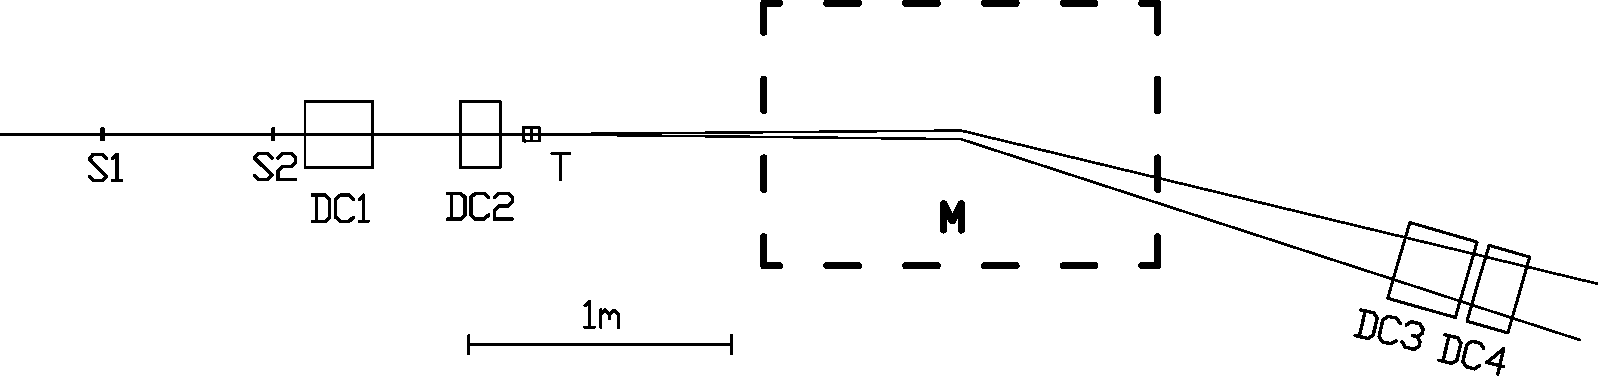
\includegraphics[width=1.00\textwidth]{STRELA_layout.pdf}
  \caption{\DIFaddFL{Schematic layout of the experimental setup to study the }\dpchex
    \DIFaddFL{charge exchange channel, consisting of scintillator counters (S1~--~S3),
    drift chambers (DC1 -- DC4), analyzing magnet M and target T.}}
  \label{fig:STRELA_layout}
\end{figure*}

\DIFaddend Based on the above mentioned ideas and experimental results, obtained using the
\DIFdelbegin \DIFdel{one meter }\DIFdelend \DIFaddbegin \DIFadd{1m }\DIFaddend HBC \cite{gla02,gla08}, the experiment STRELA has been designed and
constructed in the Veksler Baldin Laboratory for High Energy Physics (VBLHEP) of
the Joint Institute for Nuclear Research (JINR) in Dubna with the aim to select
and detect charge exchange events in deuteron proton collisions. The experiment
demands registration of two \DIFaddbegin \DIFadd{final state }\DIFaddend protons with momenta approximately equal
to the half of the primary deuteron beam momenta. STRELA is a typical one arm
magnetic spectrometer\DIFdelbegin \DIFdel{composed }\DIFdelend \DIFaddbegin \DIFadd{, consisting }\DIFaddend of scintillator detectors \DIFaddbegin \DIFadd{(}\DIFaddend S1 \DIFdelbegin \DIFdel{, S2 }\DIFdelend \DIFaddbegin \DIFadd{-- S3) }\DIFaddend used to
trigger the setup\DIFdelbegin \DIFdel{and }\DIFdelend \DIFaddbegin \DIFadd{, }\DIFaddend blocks of drift chambers (DC1 -- DC4) used as coordinate
detector\DIFdelbegin \DIFdel{and
}\DIFdelend \DIFaddbegin \DIFadd{, }\DIFaddend analyzing magnet M \DIFdelbegin \DIFdel{. The recent version of the experimental setup is shown in
Fig.}\DIFdelend \DIFaddbegin \DIFadd{and targets (C and CH$_2$), see
Fig.~}\DIFaddend \ref{fig:STRELA_layout}.

\DIFdelbegin %DIFDELCMD < \begin{figure*}[t] %%%
%DIF <  two-column wide
  %DIFDELCMD < \centering
%DIFDELCMD <   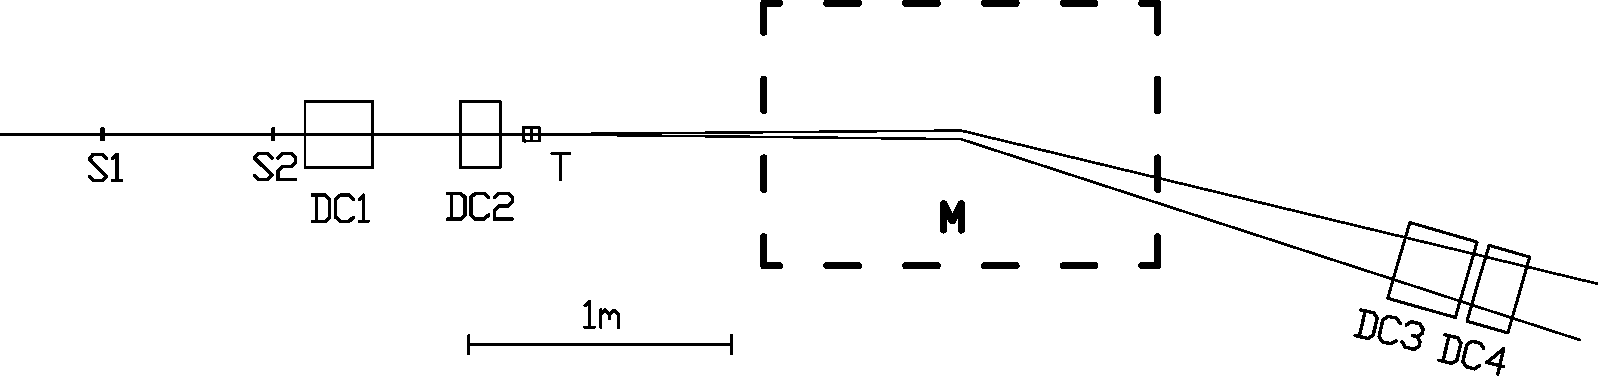
\includegraphics[width=1.00\textwidth]{STRELA_layout.pdf}
%DIFDELCMD <   %%%
%DIFDELCMD < \caption{%
{%DIFAUXCMD
\DIFdelFL{Layout of the experimental setup for determining the spin-dependent
    part of }%DIFDELCMD < \np %%%
\DIFdelFL{scattering: scintillator counters S1 and S2, drift chambers (DC1
    -- DC4), analyzing magnet M and target T.}}
  %DIFAUXCMD
%DIFDELCMD < \label{fig:STRELA_layout}
%DIFDELCMD < \end{figure*}
%DIFDELCMD < 

%DIFDELCMD < %%%
\DIFdelend The sensitive areas of the drift chambers are the following: 12.5 $\times$ 12.5
cm$^2$ for DC1, DC2 (small chambers) and 25 $\times$ 25 cm$^2$ for DC3, DC4
(large chambers). The right handed coordinate system has been used, where the
$z$ axis is in the beam direction and $x$ and $y$ axis lie in the plane of the
chambers. \DIFdelbegin \DIFdel{All }\DIFdelend \DIFaddbegin \DIFadd{Drift }\DIFaddend chambers contain an (Ar\DIFdelbegin \DIFdel{$_2$}\DIFdelend \DIFaddbegin \DIFadd{\,+\,}\DIFaddend CH$_4$) gas mixture and have
alternating, orthogonal $x$ and $y$ coordinate planes. Chambers DC1, DC3, DC4
are \DIFdelbegin \DIFdel{equiped }\DIFdelend \DIFaddbegin \DIFadd{equipped }\DIFaddend with $xy$ wires and DC2 only with $x$ wires. DC1 and DC3 are
composed of 8 sensitive planes ($4y$, $4x$), DC4 is composed of 4 sensitive
planes ($2y$, $2x$) while the DC2 contains 4 sensitive planes ($4x$).
\DIFdelbegin \DIFdel{The
analyzing magnet M of field intensity $B = 0.85$ T is used to separate deuterons
and two protons, respectively.
}\DIFdelend 

The drift length for all chambers is $r_{max} = 21$ mm. The basic
characteristics of the drift chambers have been established from irradiation of
a polyethylene target with a deuteron beam of 3.5 \GeVc momentum. For each wire
the minimal $t_{min}$ and maximal $t_{max}$ drift times have been
determined. The average total drift time was found to be $\sim$~450~ns. In the
track finding procedure the relation between the measured drift time and the
minimal distance from the anode wire to the track plays an important role. To
find the function, transforming the drift time $t$ to radius $r$, also referred
to as $r(t)$ relation, is the central task. This transformation function may
depend on many parameters like: the electric field strength, the gas mixture,
the pressure, the temperature and the drift chamber geometry. For determination
of the transformation function two methods are applied: the linear or quick one,
mainly used for the preliminary results and online monitoring, the second
method, called cumulative or integral one suitable for offline purposes, which
gives the final results. The spatial resolution of the drift chambers used in
the STRELA setup is in the range of $\sim$~80\,--120~$\muup$m
% \muup (or \upmu) not for mathptmx
(Fig.~\ref{fig:res_chambers}). \DIFaddbegin \DIFadd{The minimal time between consecutive signals is
$\sim$~50 ns, which corresponds to a minimum distance of $\sim$~2 mm between the
tracks in the drift chamber, which fully satisfies the requirement of the STRELA
experiment. Moreover, the analyzing magnet enhances the space separation of the
recorded protons from the examined reaction. }\DIFaddend More technical details and the
algorithm of the track reconstruction can be found in \cite{gla13}.

\DIFdelbegin %DIFDELCMD < \begin{figure}[ht]
%DIFDELCMD <   %%%
\DIFdelendFL \DIFaddbeginFL \begin{figure}[t]
  \DIFaddendFL \centering
  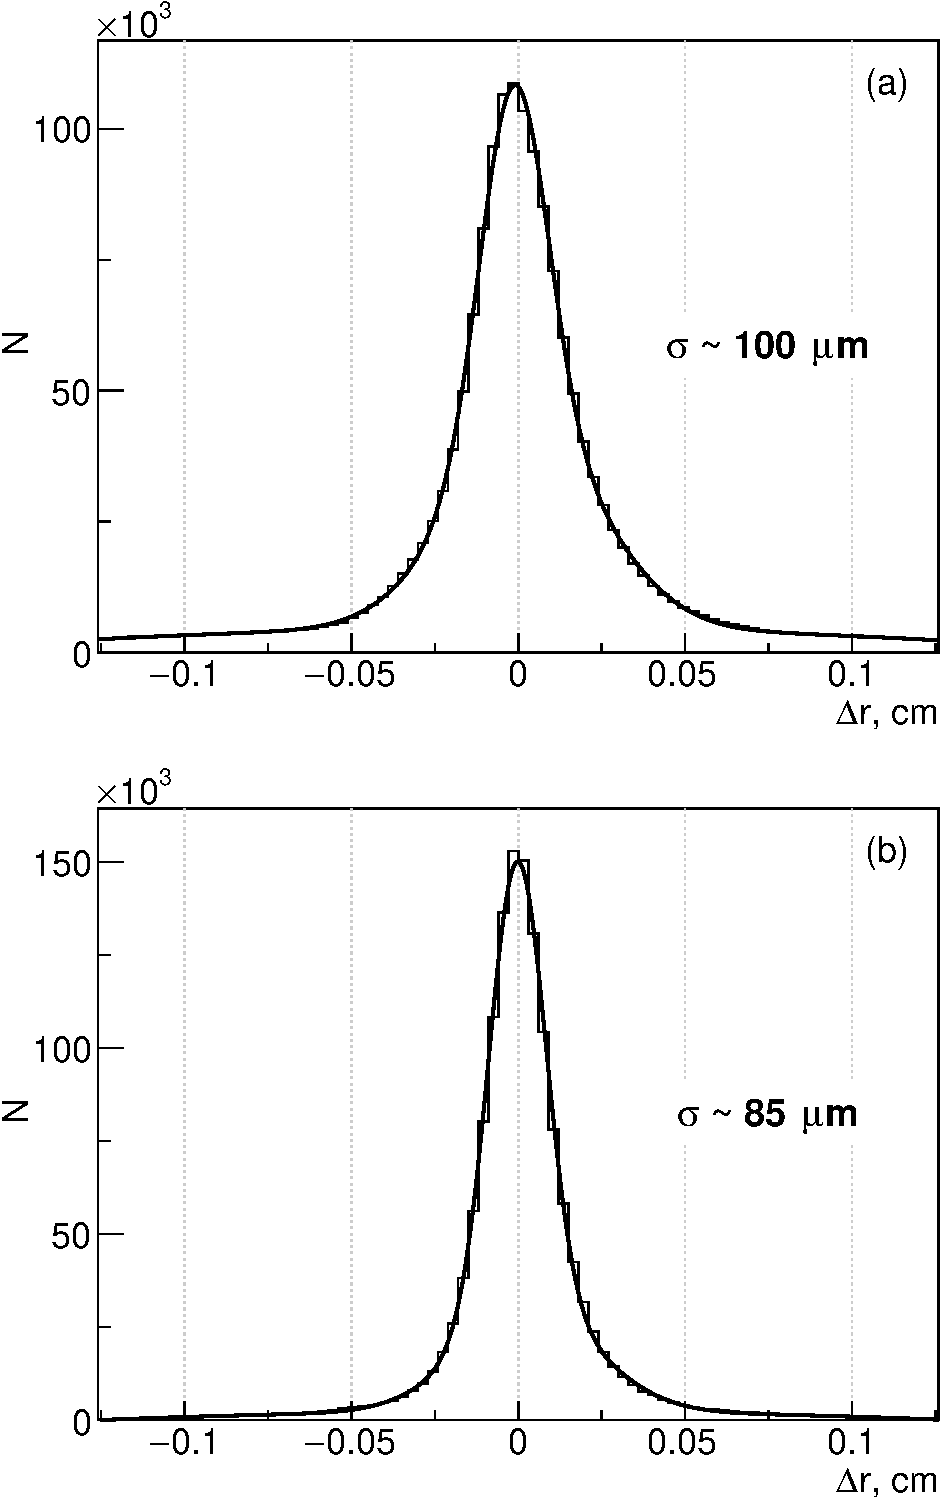
\includegraphics[width=0.48\textwidth]{res_chambers.pdf}
  \caption{Example of distribution of track residuals $\Delta r$ in the $xz$
    plane of drift chambers: (a) small and (b) large. The solid curve is a
    double Gaussian approximation \DIFaddbeginFL \DIFaddFL{\cite{gla13}}\DIFaddendFL .}
  \label{fig:res_chambers}
\end{figure}

The experimental setup was started by \DIFdelbegin \DIFdel{the two polysty\-rene based }\DIFdelend \DIFaddbegin \DIFadd{coincidence of two }\DIFaddend scintillation counters
S1 (dimensions \DIFdelbegin \DIFdel{10 }\DIFdelend \DIFaddbegin \DIFadd{7.5 }\DIFaddend $\times$ \DIFdelbegin \DIFdel{10 }\DIFdelend \DIFaddbegin \DIFadd{7.5 }\DIFaddend $\times$ 0.5 cm$^3$) and S2 (dimensions \DIFdelbegin \DIFdel{7
}\DIFdelend \DIFaddbegin \DIFadd{diameter
3.0 }\DIFaddend $\times$ \DIFdelbegin \DIFdel{7 $\times$ 0.5 }\DIFdelend \DIFaddbegin \DIFadd{0.2 }\DIFaddend cm$^3$). The \DIFdelbegin \DIFdel{light guides are made of plexiglass. For
light readout XP 2020 photomultipliers were used. The }\DIFdelend signals from the \DIFaddbegin \DIFadd{XP 2020 }\DIFaddend photomultipliers are
connected to the \DIFdelbegin \DIFdel{shaper inputs. The use of these shapers allows }\DIFdelend \DIFaddbegin \DIFadd{shapers with constant fraction timing in order }\DIFaddend to compensate
the time \DIFdelbegin \DIFdel{spread of the signals caused by the leading edge
of the amplitude of the photomultiplier }\DIFdelend \DIFaddbegin \DIFadd{jitter of the amplitude }\DIFaddend signal. The time and amplitude information from
the counters is digitized and recorded in each event for the subsequent
monitoring of the counters and the entire trigger system functionality.
\DIFdelbegin \DIFdel{The trigger system of the setup must ensure selection of events
of the deuteron breakup reaction at zero angle (or close to zero) between the
incoming deuteron and scattering protons. The acceptance of the experimental
facility for the studied process of charge exchange reaction is close to 100~\%.
}\DIFdelend 

The dipole electromagnet 2SP-40, with transverse dimensions 100 $\times$ 30
cm$^2$ \DIFdelbegin \DIFdel{, was used as an analyzing magnet. The magnet }\DIFdelend \DIFaddbegin \DIFadd{and length 150 cm, }\DIFaddend creates the required magnetic field \DIFdelbegin \DIFdel{in the range of \,0.7~--~1.0 T at a distance of 150 cm along the
path of the particles. The spreads in space of the non interacting deuteron beam
and that of the recorded protons from the examined reaction are bended to the
blocks of large drift chambers for detection. The radius of the curvature of the
stripping protons trajectory in the magnet is about 7 m at the value of the
magnetic field 0.83 T.
}%DIFDELCMD < 

%DIFDELCMD < %%%
\DIFdel{The STRELA setup is irradiated with a deuteron beam of an incident momentum of
3.5 }%DIFDELCMD < \GeVc%%%
\DIFdel{. The detected events are supposed to contain either two protons with
close momenta (equal to the }\DIFdelend \DIFaddbegin \DIFadd{0.85 T and serves
as an analyzing magnet. The recorded protons of about the }\DIFaddend half of the incident
deuteron beam \DIFdelbegin \DIFdel{momenta), from the charge exchange reaction of a deuteron with a proton }%DIFDELCMD < \dpchex %%%
\DIFdel{or a single
proton from the charge retention deuteron breakup }%DIFDELCMD < \dpret%%%
\DIFdel{. The extracted beam
intensity from the accelerator is not lower then $\sim 10^{7}$ particles per
spill. Since the drift chambers are operable at intensities lower than
$\sim 10^{6}$ particles/spill, a steel collimator with a rectangular aperture of
4 $\times$ 4 mm$^2$ and a length of 1.2 m has to
be used to reduce the intensity. After applying the collimator the deuteron beam intensity of $\sim 5\times10^5$ particles per spill or below is reached at the target. The
deuteron flux (number of triggers) has been determined using S1 and S2
scintillation counters (monitored numbers) in coincidence. This is corrected for }\DIFdelend \DIFaddbegin \DIFadd{momentum from the examined reaction are bended at 0.289 mrad to
}\DIFaddend the \DIFdelbegin \DIFdel{efficiency of the drift chambersand admixture in the beam using a direct
deuteron beam. The
track of deuteron beam in drift chambers DC1, DC2 before
magnet and behind DC3, DC4 are reconstructed using the track reconstruction
algorithm \cite{gla13}. The value of the correction is
different from run to run
and is in the interval 0.85~--~0.89}\DIFdelend \DIFaddbegin \DIFadd{blocks of large drift chambers (DC3 and DC4) for detection; unscattered
primary deuteron beam does not enter the sensitive areas of these chambers}\DIFaddend . \DIFaddbegin \DIFadd{The
momentum resolution measured with the primary deuteron beam of 3.5 }\GeVc \DIFadd{is
about 1~\%.
}\DIFaddend 

Carbon (C) and polyethylene (CH$_2$) targets \DIFdelbegin \DIFdel{have been }\DIFdelend \DIFaddbegin \DIFadd{are }\DIFaddend used to extract the $dp$
interaction \DIFdelbegin \DIFdel{. Carbon target was used to account for the background events. The
final distributions of the $dp$ interactions are obtained }\DIFdelend by subtracting CH$_2$ and C distributions. The \DIFdelbegin \DIFdel{size }\DIFdelend \DIFaddbegin \DIFadd{volume }\DIFaddend of the targets
\DIFdelbegin \DIFdel{have been }\DIFdelend \DIFaddbegin \DIFadd{is }\DIFaddend determined by carbon nuclei equivalent. \DIFdelbegin \DIFdel{The shape of targets CH$_2$ and C }\DIFdelend \DIFaddbegin \DIFadd{Their shapes }\DIFaddend are cylindrical, both
with diameters of 60 mm. The length of targets CH$_2$ and C are 48\DIFaddbegin \DIFadd{~}\DIFaddend mm and 54\DIFaddbegin \DIFadd{~}\DIFaddend mm,
respectively. The density of H nuclei per\DIFaddbegin \DIFadd{~}\DIFaddend cm$^2$ for CH$_2$ target is (4.74
$\pm$ 0.05)$\times$10$^{23}$ cm$^{-2}$.
\DIFdelbegin \DIFdel{The background from other channels of the $dp$ reactionand the influence of carbon nuclei have been }\DIFdelend \DIFaddbegin 

\DIFadd{The measurement was done at the intensities of beam of 2~--~3~$\times$~10$^5$
deuterons per second, duration of the spill was 4~seconds. The deuteron flux
(number of triggers) has been determined by S1 and S2 scintillation counters in
coincidence. This is corrected for the inefficiency of the drift chambers and
admixture of protons in the primary deuteron beam using the empty target
measurements. The value of the correction is different from run to run and is in
the interval 0.85~--~0.89.
}

\DIFadd{The trigger system selects events of the deuteron breakup reaction, where at
least one charged track inclined by magnet reaches the drift chambers DC3 and
DC4. The momenta of the tracks in the event are reconstructed using information
from the magnet and from the drift chambers. Into the analy\-sis only the events
containing two reconstructed tracks are involved.
}

\DIFadd{The detector performance for two-track events was }\DIFaddend estimated by the use of the
GEANT3 \DIFdelbegin \DIFdel{simulation }\DIFdelend package for transporting the \DIFdelbegin \DIFdel{reaction products (taken from the corresponding events of the one meter bubble chamber at the
momenta 3.35 }%DIFDELCMD < \GeVc%%%
\DIFdel{) through the }\DIFdelend \DIFaddbegin \DIFadd{$dp$ interaction products from the 1m HBC
events through the STRELA }\DIFaddend experimental setup. \DIFdelbegin \DIFdel{More details about the chamber experiment can be found in \cite{gla02,gla08}. There is also shown that the }%DIFDELCMD < \dpchex %%%
\DIFdel{reaction proceeding predominantly as a quasi free nucleon
interaction and intermediate isobaric states does not influence the differential
cross section at $t = 0$}\DIFdelend \DIFaddbegin \DIFadd{The plots of momenta
$p_1$~\textit{vs.}~$p_2$ of the two charged particles reaching the DC3 and DC4
chambers are shown in Fig. \ref{fig:p1vsp2_sim}. Simulation including all $dp$
interaction channels (a) and }\dpfrag \DIFadd{channel only (b). From this comparison and
the fact that 1m HBC is full solid angle detector one can judge that the two
protons of the charge exchange reaction are fully in the detector acceptance}\DIFaddend .

\DIFaddbegin \begin{figure}[t]
  \centering
  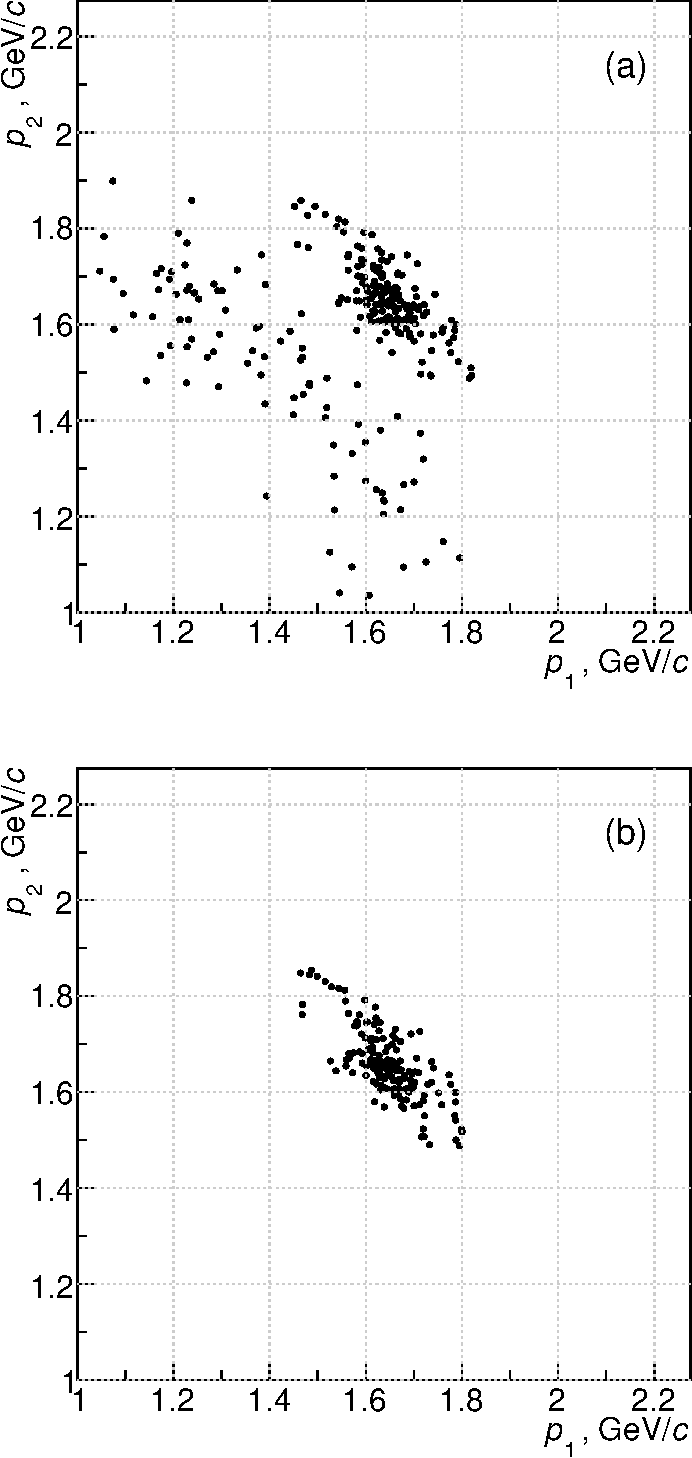
\includegraphics[width=0.43\textwidth]{p1_vs_p2_1.pdf}
  \caption{\DIFaddFL{Plot of the GEANT3 tracked 1m HBC two charged particles momenta $p_1$
    \textit{vs.} $p_2$ from $dp$: all channels (a) and }\dpfrag \DIFaddFL{only~(b).}}
  \label{fig:p1vsp2_sim}
\end{figure}

\DIFaddend \section{Data analysis and experimental results}
The experimental facility has been irradiated in the beam of deuterons with 3.5
\GeVc momenta and \DIFdelbegin \DIFdel{one billion triggers were received}\DIFdelend \DIFaddbegin \DIFadd{approximately milliard triggers were taken}\DIFaddend . The first step in
the analysis was to decode events. Calibration procedure and the track
reconstruction in the drift chambers transformed the raw data into physical
quantities. For the further processing and physical analysis three \DIFdelbegin \DIFdel{tracks }\DIFdelend \DIFaddbegin \DIFadd{track
segments }\DIFaddend in the $xz$ plane \DIFaddbegin \DIFadd{drift chambers }\DIFaddend were selected: one before the target
and two behind it. The topology of this events is shown in
Fig. \ref{fig:STRELA_layout}. \DIFaddbegin \DIFadd{The momentum of the particles (protons) was
determined from the angle of deflection of the charged particle after passing
through the magnet M.
}\DIFaddend 

\DIFaddbegin \DIFadd{The }\dpfrag \DIFadd{events reaching the drift chambers DC3 and DC4 are supposed to
contain: two fast protons from the charge exchange reaction }\dpchex \DIFadd{with momenta
approximately equal to the half of the beam momenta, or a single fast proton
from the charge retention }\dpret \DIFadd{channel, where the recoil slow proton is
filtered out by the magnet.
}

\DIFadd{In the presented data (Fig. \ref{fig:p1vsp2_exp}) two well-separated areas can
be distinguished as well as in the simulated ones
(Fig.~\ref{fig:p1vsp2_sim}~(a)). The more populated ellipse like area in
Fig. \ref{fig:p1vsp2_sim}~(a) can be ascribed to the charge exchange events if
one compares with the results of simulation in
Fig. \ref{fig:p1vsp2_sim}~(b). This crosschecks the statements made about the
detector acceptance above. The arch like areas in Fig. \ref{fig:p1vsp2_sim}~(a)
and Fig. \ref{fig:p1vsp2_exp} correspond to background two-track events. A
simple cut on the sum of the two reconstructed momenta can remove the events
from the arch like area.
}

\DIFaddend \begin{figure}[h]
  \centering
  \DIFdelbeginFL %DIFDELCMD < 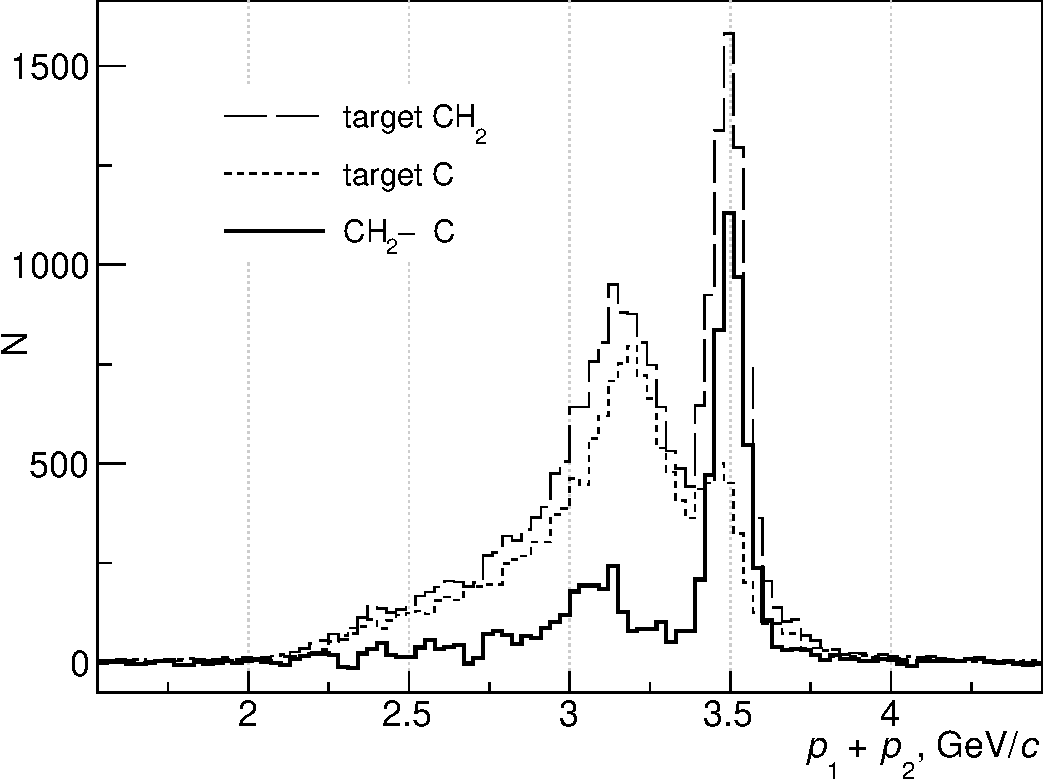
\includegraphics[width=0.48\textwidth]{p1_plus_p2_1.pdf}
%DIFDELCMD <   %%%
\DIFdelendFL \DIFaddbeginFL 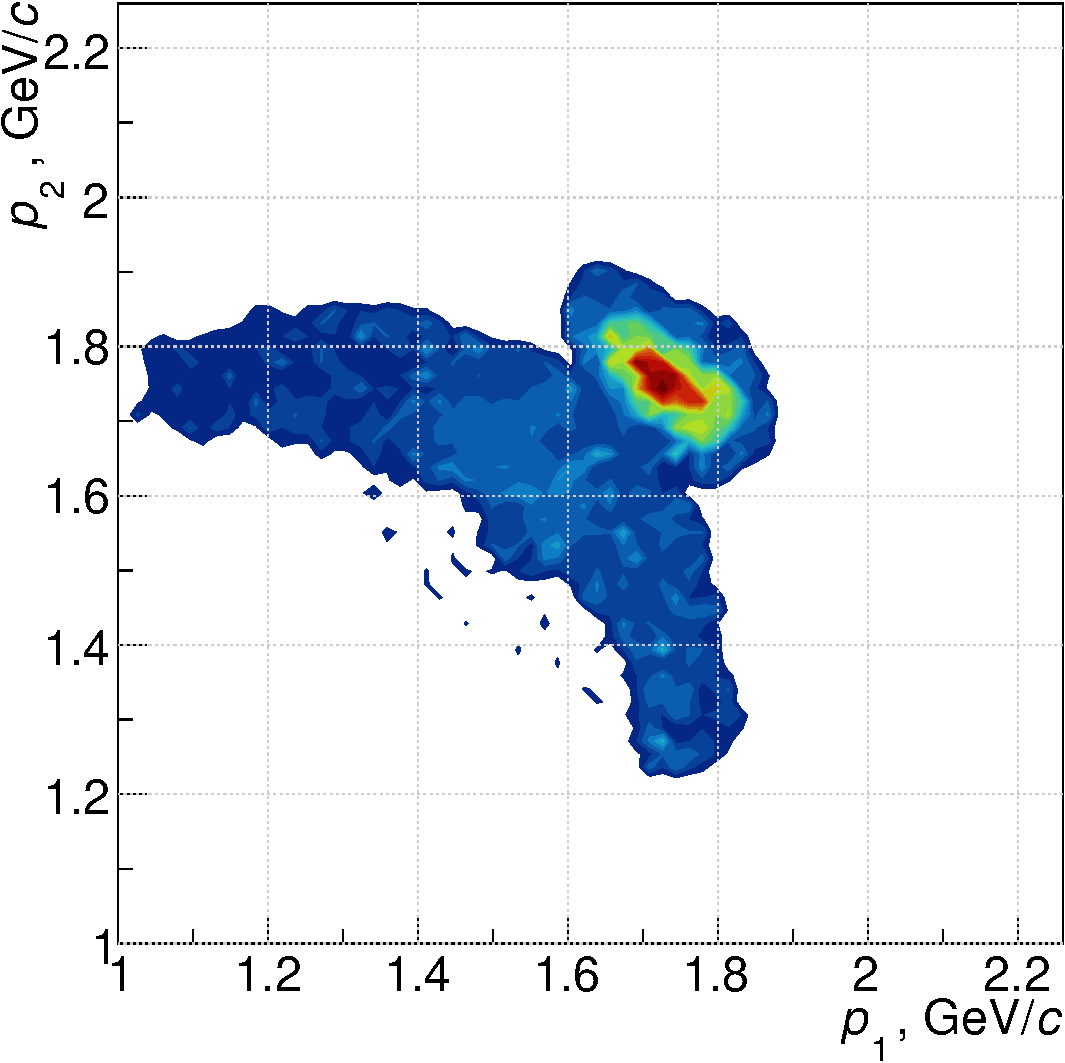
\includegraphics[width=0.43\textwidth]{p1_vs_p2_2.pdf}
  \DIFaddendFL \caption{\DIFdelbeginFL \DIFdelFL{Distributions }\DIFdelendFL \DIFaddbeginFL \DIFaddFL{Plot }\DIFaddendFL of the \DIFdelbeginFL \DIFdelFL{sum }\DIFdelendFL \DIFaddbeginFL \DIFaddFL{measured momenta $p_1$ \textit{vs.} $p_2$ }\DIFaddendFL of the two
    \DIFdelbeginFL \DIFdelFL{protons momenta }\DIFdelendFL \DIFaddbeginFL \DIFaddFL{tracks }\DIFaddendFL from \DIFdelbeginFL \DIFdelFL{$dp$
    reaction, experimental results: (a) target }\DIFdelendFL \DIFaddbeginFL \DIFaddFL{$d$ + }\DIFaddendFL CH\DIFdelbeginFL \DIFdelFL{$_2$ full line}\DIFdelendFL \DIFaddbeginFL \DIFaddFL{$_{2}$ interaction}\DIFaddendFL , \DIFdelbeginFL \DIFdelFL{target C dashed
    line, (b) difference between CH$_2-$\,C targets}\DIFdelendFL \DIFaddbeginFL \DIFaddFL{experimental result}\DIFaddendFL .}
  \DIFdelbeginFL %DIFDELCMD < \label{fig:p1p2exp}
%DIFDELCMD < %%%
\DIFdelendFL \DIFaddbeginFL \label{fig:p1vsp2_exp}
\DIFaddendFL \end{figure}

The \DIFaddbegin \DIFadd{obtained }\DIFaddend distribution of the sum of the two charged particles (two protons)
momenta for both \DIFdelbegin \DIFdel{targets are obtained. The background from C and }\DIFdelend CH$_2$ \DIFdelbegin \DIFdel{targets can be
neglected. The dependences of the sum of the two proton momenta from $dp$
reaction are presented }\DIFdelend \DIFaddbegin \DIFadd{and C targets are displayed }\DIFaddend in Fig. \ref{fig:p1p2exp}\DIFdelbegin \DIFdel{for CH$_2$ and C targets (a)
and their difference CH$_2-\,$C (b) }\DIFdelend \DIFaddbegin \DIFadd{,
distinguished by long dashed and dashed lines, respectively. The difference of
the two distributions (full line) shows that the background from C target can be
reduced}\DIFaddend . The results of simulation \DIFdelbegin \DIFdel{(Fig.\ref{fig:p1p2sim}) }\DIFdelend \DIFaddbegin \DIFadd{shown in Fig.~\ref{fig:p1p2sim} }\DIFaddend include all
channels \DIFaddbegin \DIFadd{of the }\DIFaddend $dp$ \DIFdelbegin \DIFdel{reaction }\DIFdelend \DIFaddbegin \DIFadd{interaction }\DIFaddend (a) and \DIFdelbegin \DIFdel{channel
}\DIFdelend \dpfrag \DIFaddbegin \DIFadd{channel }\DIFaddend only (b). Note that for
the simulation real events \DIFdelbegin \DIFdel{from the one meter
bubble chamber }\DIFdelend \DIFaddbegin \DIFadd{(with relatively small statistics) from the 1m HBC }\DIFaddend at
the momenta 3.35~\GeVc \DIFdelbegin \DIFdel{(with relatively small statistics) }\DIFdelend were used. As one can see, the distribution has a
characteristic peak near the incoming deuteron momentum kinematically associated
with the pair of protons from the \dpfrag reaction (Fig. \ref{fig:p1p2exp}\DIFdelbegin \DIFdel{(b)).
The contribution from
the background reactions, other than the studied }%DIFDELCMD < \dpfrag %%%
\DIFdel{reaction, which could
also produce the two positively charged track in the forward direction, is
negligible (Fig. \ref{fig:p1p2sim} (b)). Into the differential cross section
$d\sigma/dt$ }\DIFdelend \DIFaddbegin \DIFadd{).
Into the further analysis }\DIFaddend only those events have been included, where the sum of
the two \DIFdelbegin \DIFdel{charged particle }\DIFdelend \DIFaddbegin \DIFadd{protons }\DIFaddend momenta is in the interval (3.5 $\pm$ 0.2) \GeVc\DIFdelbegin \DIFdel{(Fig.
\ref{fig:p1p2exp} (b)).
}\DIFdelend \DIFaddbegin \DIFadd{.
}\DIFaddend 

\DIFdelbegin %DIFDELCMD < \begin{figure}[h]
%DIFDELCMD <   %%%
\DIFdelendFL \DIFaddbeginFL \begin{figure}[t]
  \DIFaddendFL \centering
  \DIFdelbeginFL %DIFDELCMD < 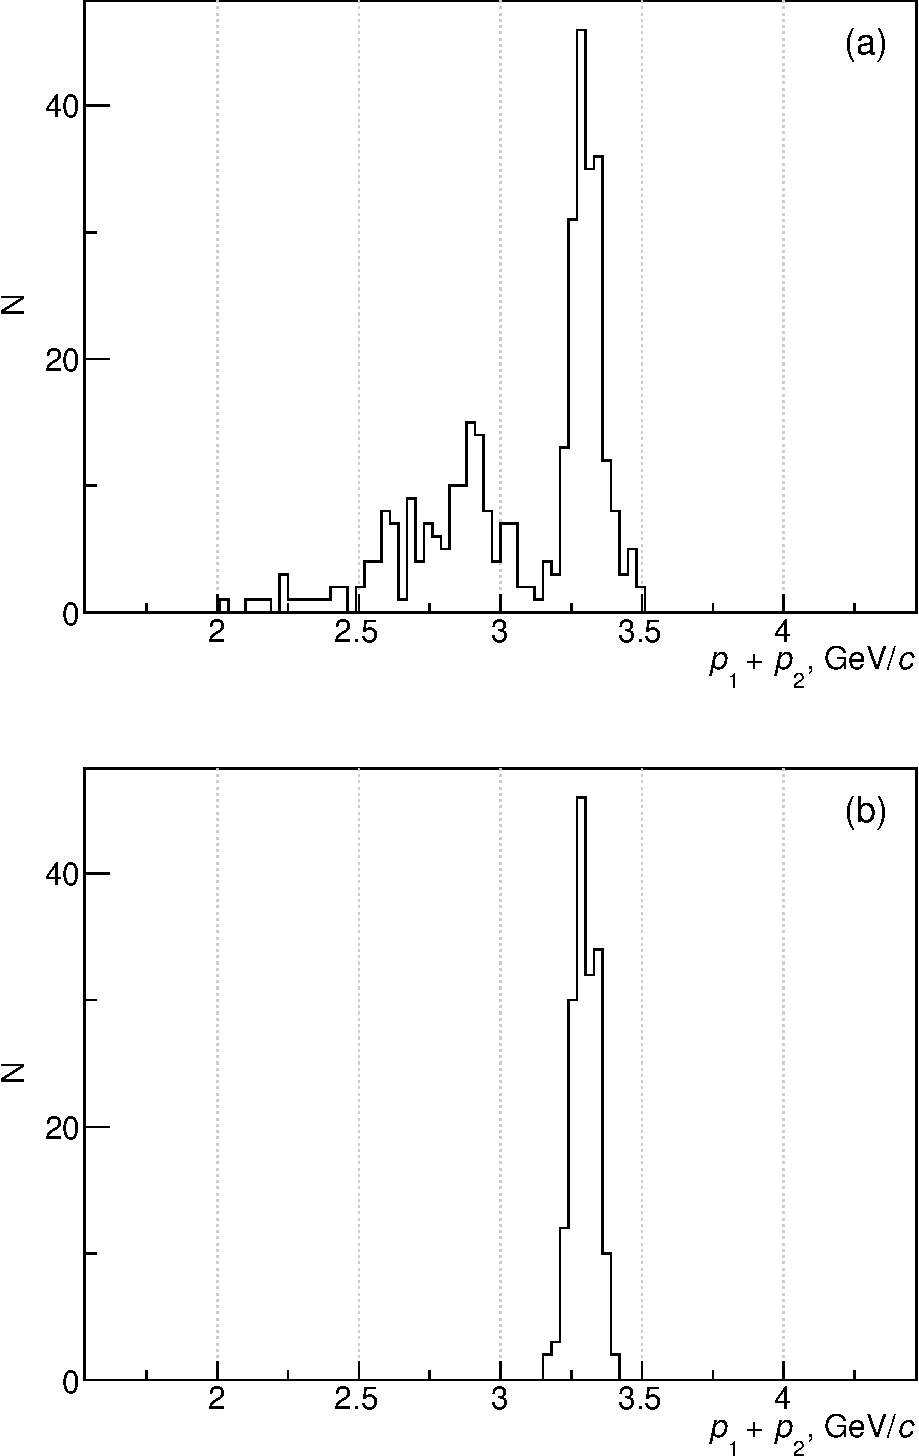
\includegraphics[width=0.48\textwidth]{p1_plus_p2_2.pdf}
%DIFDELCMD <   %%%
\DIFdelendFL \DIFaddbeginFL 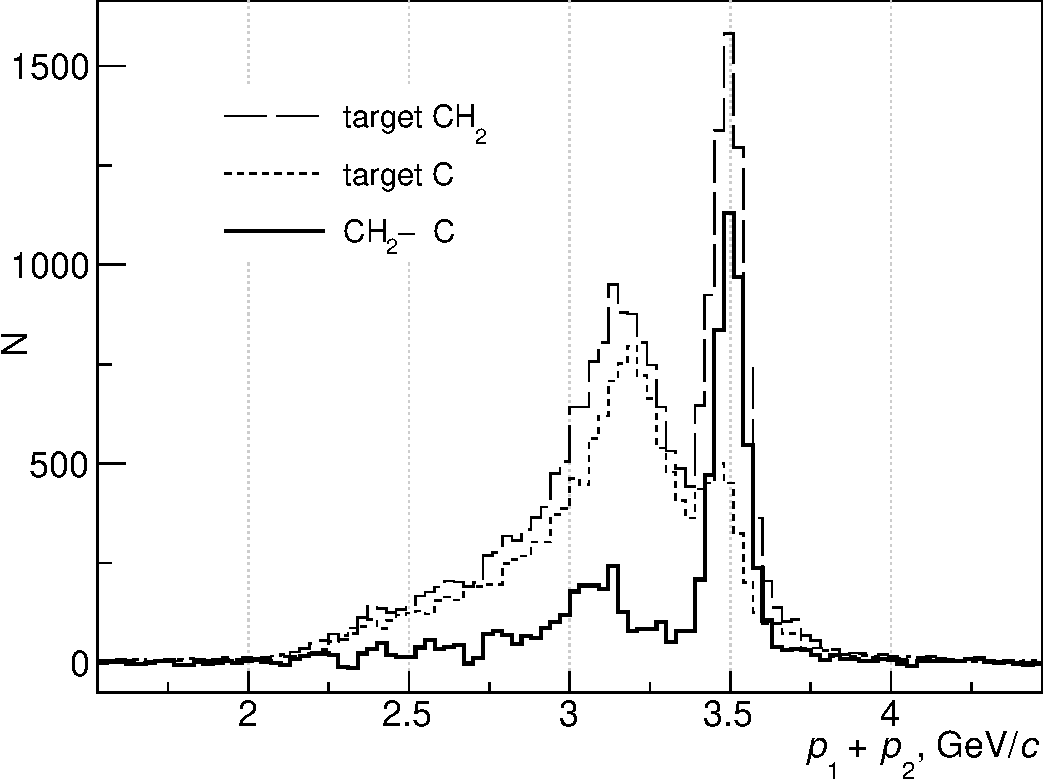
\includegraphics[width=0.43\textwidth]{p1_plus_p2_1.pdf}
  \DIFaddendFL \caption{Distributions of the sum of the two protons momenta from
    \DIFdelbeginFL \DIFdelFL{$dp$
    reaction}\DIFdelendFL \DIFaddbeginFL \DIFaddFL{$d$~+~CH$_{2}$ and $d$ + C interactions}\DIFaddendFL , \DIFdelbeginFL \DIFdelFL{simulation }\DIFdelendFL \DIFaddbeginFL \DIFaddFL{experimental }\DIFaddendFL results: \DIFdelbeginFL \DIFdelFL{(a) include all channels $dp$ reaction }\DIFdelendFL \DIFaddbeginFL \DIFaddFL{CH$_2$ target
    long dashed line, C target dashed line }\DIFaddendFL and \DIFdelbeginFL \DIFdelFL{(b)
    channel }%DIFDELCMD < \dpfrag %%%
\DIFdelFL{only}\DIFdelendFL \DIFaddbeginFL \DIFaddFL{their difference full line}\DIFaddendFL .}
  \DIFaddbeginFL \label{fig:p1p2exp}
\end{figure}
\begin{figure}[t]
  \centering
  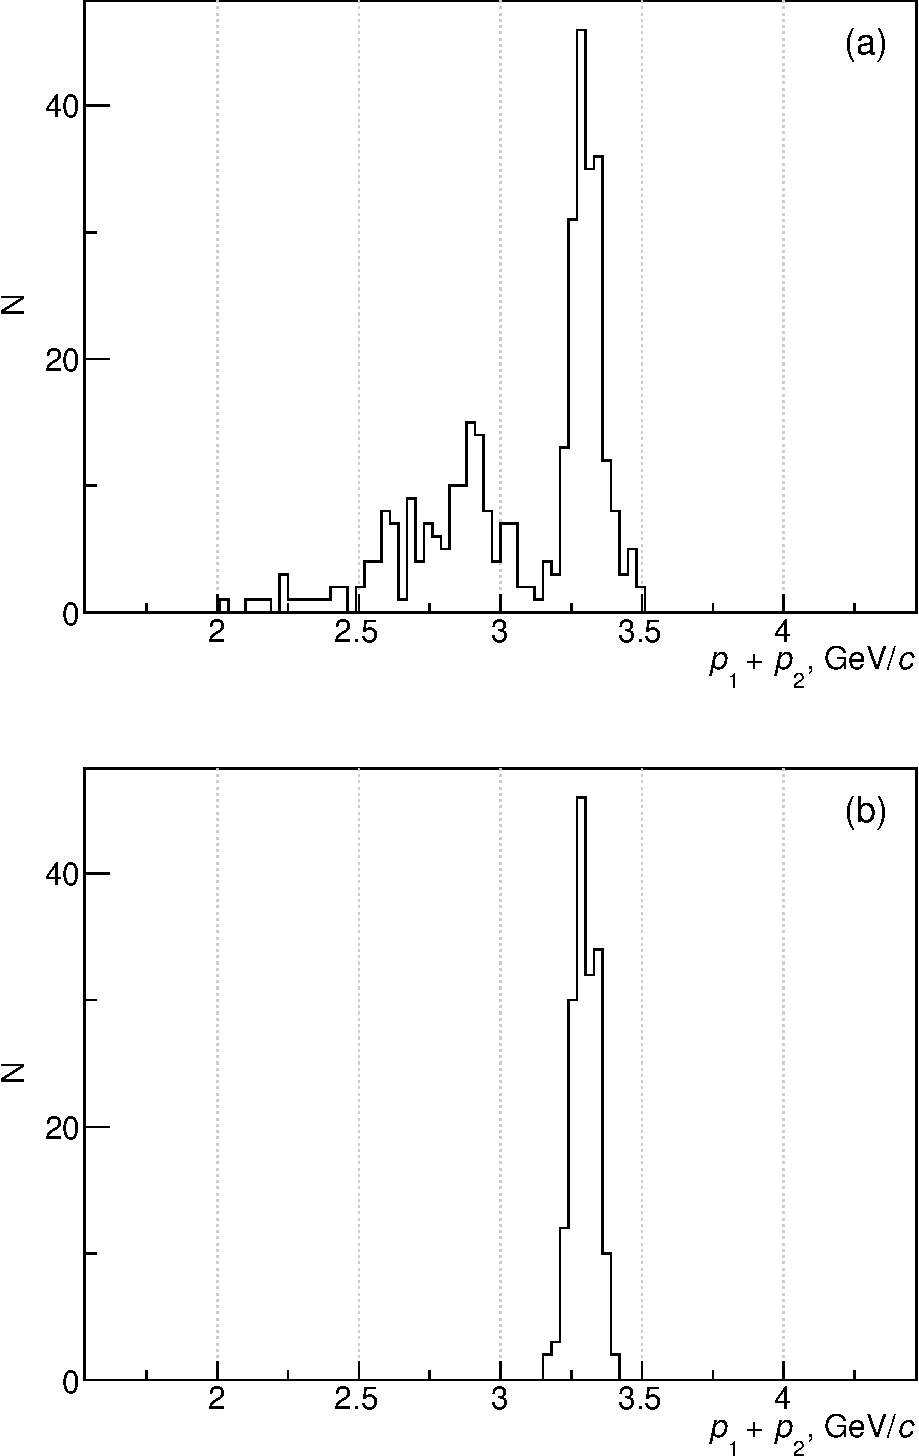
\includegraphics[width=0.43\textwidth]{p1_plus_p2_2.pdf}
  \caption{\DIFaddFL{Distributions of the sum of the two protons momenta from GEANT3
    tracked 1m HBC: $dp$ all channels (a) and }\dpfrag \DIFaddFL{channel only (b).}}
  \DIFaddendFL \label{fig:p1p2sim}
\end{figure}

The \DIFdelbegin \DIFdel{plot of momenta $p_1$ \textit{vs.} $p_2$ of the two charged particles (two
protons) from $dp$ reaction is shown in Fig. \ref{fig:p1vsp2}. From the comparison of the simulation results (a) and (c) with the experimental results
(b), it can be seen that the background from other channels of the $dp$ reaction
may be eliminated.}\DIFdelend \DIFaddbegin \DIFadd{main goal of present experiment is to determine the differential cross
section $(d\sigma/dt)|\,_{t=0}$ of }\dpchex\DIFadd{, which can only be done as an
extrapolation of the measured data to $|t|\mapsto0$. This can be connected
according to Eq.~}\eqref{eq:dp_23np} \DIFadd{with the spin-dependent part of the }\np
\DIFadd{process.
}\DIFaddend 

\DIFdelbegin %DIFDELCMD < \begin{figure}[t]
%DIFDELCMD <   \centering
%DIFDELCMD <   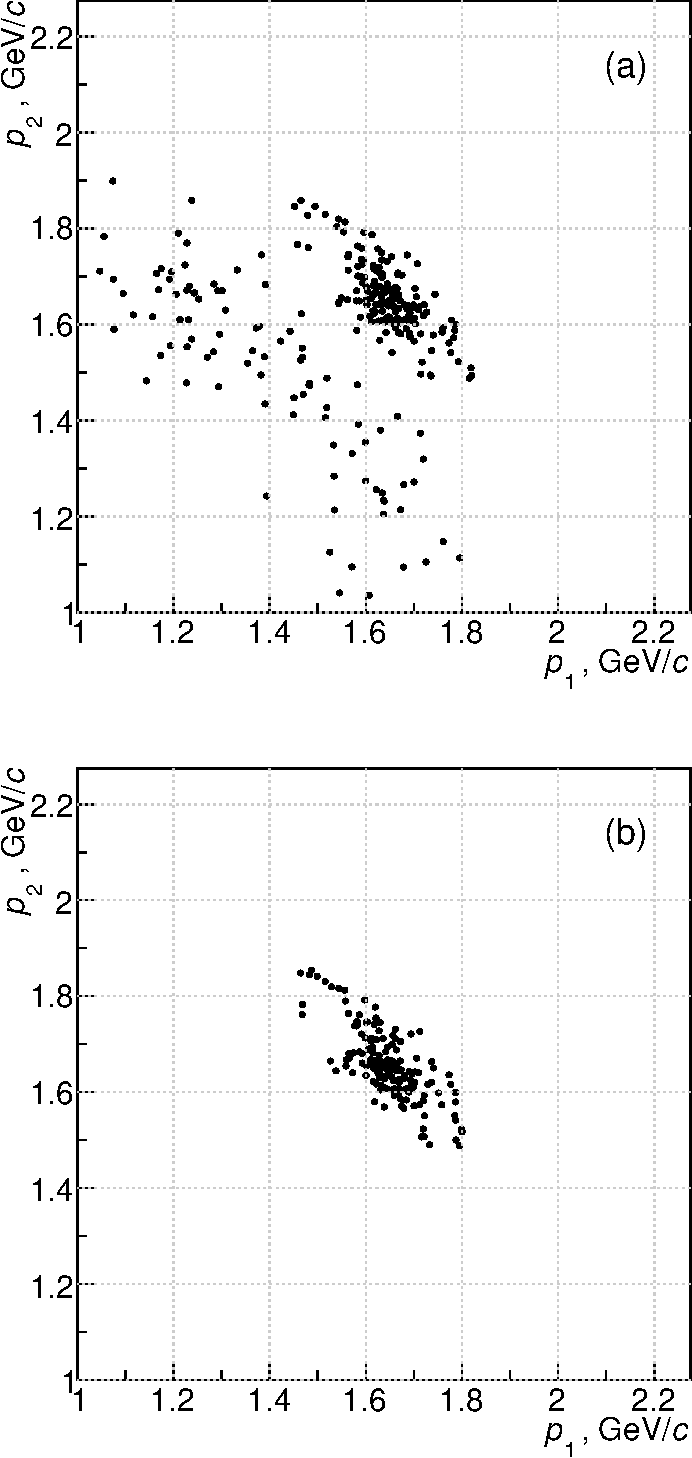
\includegraphics[width=0.41\textwidth]{p1_vs_p2_1.pdf} %%%
%DIF <  maximum width=0.41
  %DIFDELCMD < \caption{%
{%DIFAUXCMD
\DIFdelFL{Two dimensional distribution of the measured momenta $p_1$
    \textit{vs.} $p_2$ of the two protons from $dp$ reaction: (a) simulation
    includes all channels $dp$ reaction, (c) simulation only }%DIFDELCMD < \dpfrag %%%
\DIFdelFL{channel and
    (b) experimental distribution.}}
  %DIFAUXCMD
%DIFDELCMD < \label{fig:p1vsp2}
%DIFDELCMD < \end{figure}
%DIFDELCMD < 

%DIFDELCMD < %%%
\DIFdel{The measured differential distribution $dN\,/\,dt$ }\DIFdelend \DIFaddbegin \DIFadd{The measured $dN/dt$ distribution }\DIFaddend of the \dpchex reaction is displayed in
Fig. \ref{fig:dndt} together with the curve corresponding to \DIFdelbegin \DIFdel{fit by
expression
}\DIFdelend \DIFaddbegin \DIFadd{a fit by
empirically well established expression
}\DIFaddend \begin{equation}
  \DIFdelbegin %DIFDELCMD < \label{eq:dndtfit}
%DIFDELCMD <   %%%
\DIFdelend dN/dt = a\,\exp(b\,t)\,,
  \DIFaddbegin \label{eq:dndtfit}
\DIFaddend \end{equation}
with parameters \DIFdelbegin \DIFdel{$a=(435.6\,\pm\,6.8)$ and $b=(-440.9\,\pm\,9.1)$}\DIFdelend \DIFaddbegin \DIFadd{$a=(435.6 \pm 6.8)$ and $b=(-440.9 \pm 9.1)$}\DIFaddend . The value
\DIFaddbegin \DIFadd{$(dN/dt)|\,_{t=0}$ was transformed to cross section
}\begin{equation}
  \DIFadd{\frac{d\sigma}{dt}\Big|_{\,t=0} =
  \frac{a}{n\,l\,b_w}\ln\bigg(\frac{N_0}{N_0-N_{rec}}\bigg)\,,
}\end{equation}
\DIFadd{where $n$ is the number of H nuclei in cm$^{-3}$ in target, $l$ is the target
length in cm, $b_w$ is the histogram bin width. The number of reconstructed two
proton events $N_{rec}$ and the number of incoming deuterons $N_0$ were
corrected for the efficiency of chambers.
}

\begin{figure}[h]
  \centering
  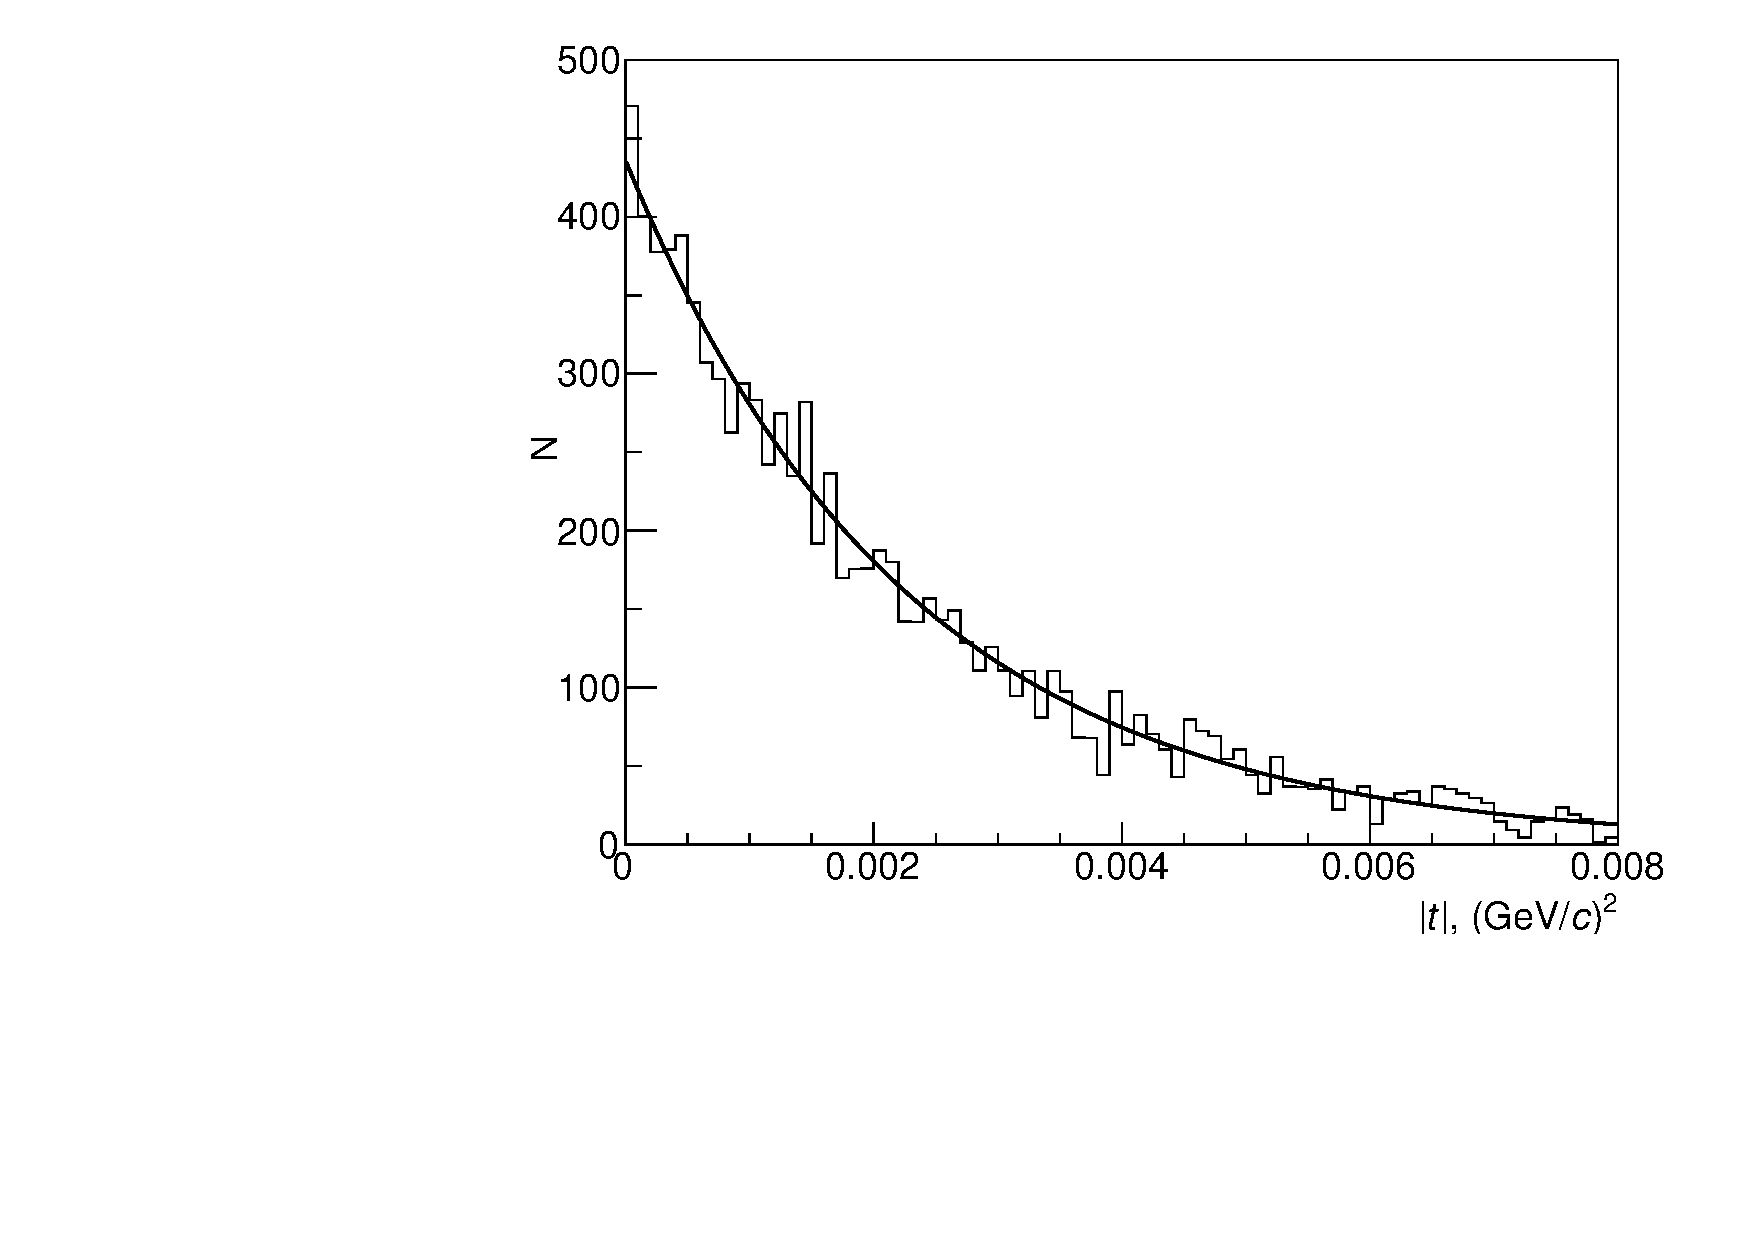
\includegraphics[width=0.48\textwidth]{dp_dN.pdf}
  \caption{\DIFaddFL{Differential distribution $dN/dt$ of the }\dpchex \DIFaddFL{reaction. The solid
    line is approximation by Eq. }\eqref{eq:dndtfit}\DIFaddFL{.}}
  \label{fig:dndt}
\end{figure}

\DIFadd{The value }\DIFaddend $(dN/dt)|\,_{t=0}=(435.6\,\pm\,6.8)$ N$/$(\GeVc)$^{\,2}$ corresponds
to the charge exchange reaction differential cross section
$(d\sigma/dt)|\,_{t=0}=(30.56\,\pm\,0.48$) mb$/$(\GeVc)$^{\,2}$.
%DIF <  3x artificial a thin space
%DIF >  3x artificial a thin space (Overfull \hbox)
The quoted \,error is statistical \,only. \,Systematic uncertainties which
affect the overall normalization of the cross sections have been estimated to be
about 5~\%. This uncertainty stems mainly from the deuteron flux determination.
The uncertainty from the target thickness and the histogram bin width are
\DIFdelbegin \DIFdel{comparably }\DIFdelend \DIFaddbegin \DIFadd{relatively }\DIFaddend small.

\DIFdelbegin %DIFDELCMD < \begin{figure}[h]
%DIFDELCMD <   \centering
%DIFDELCMD <   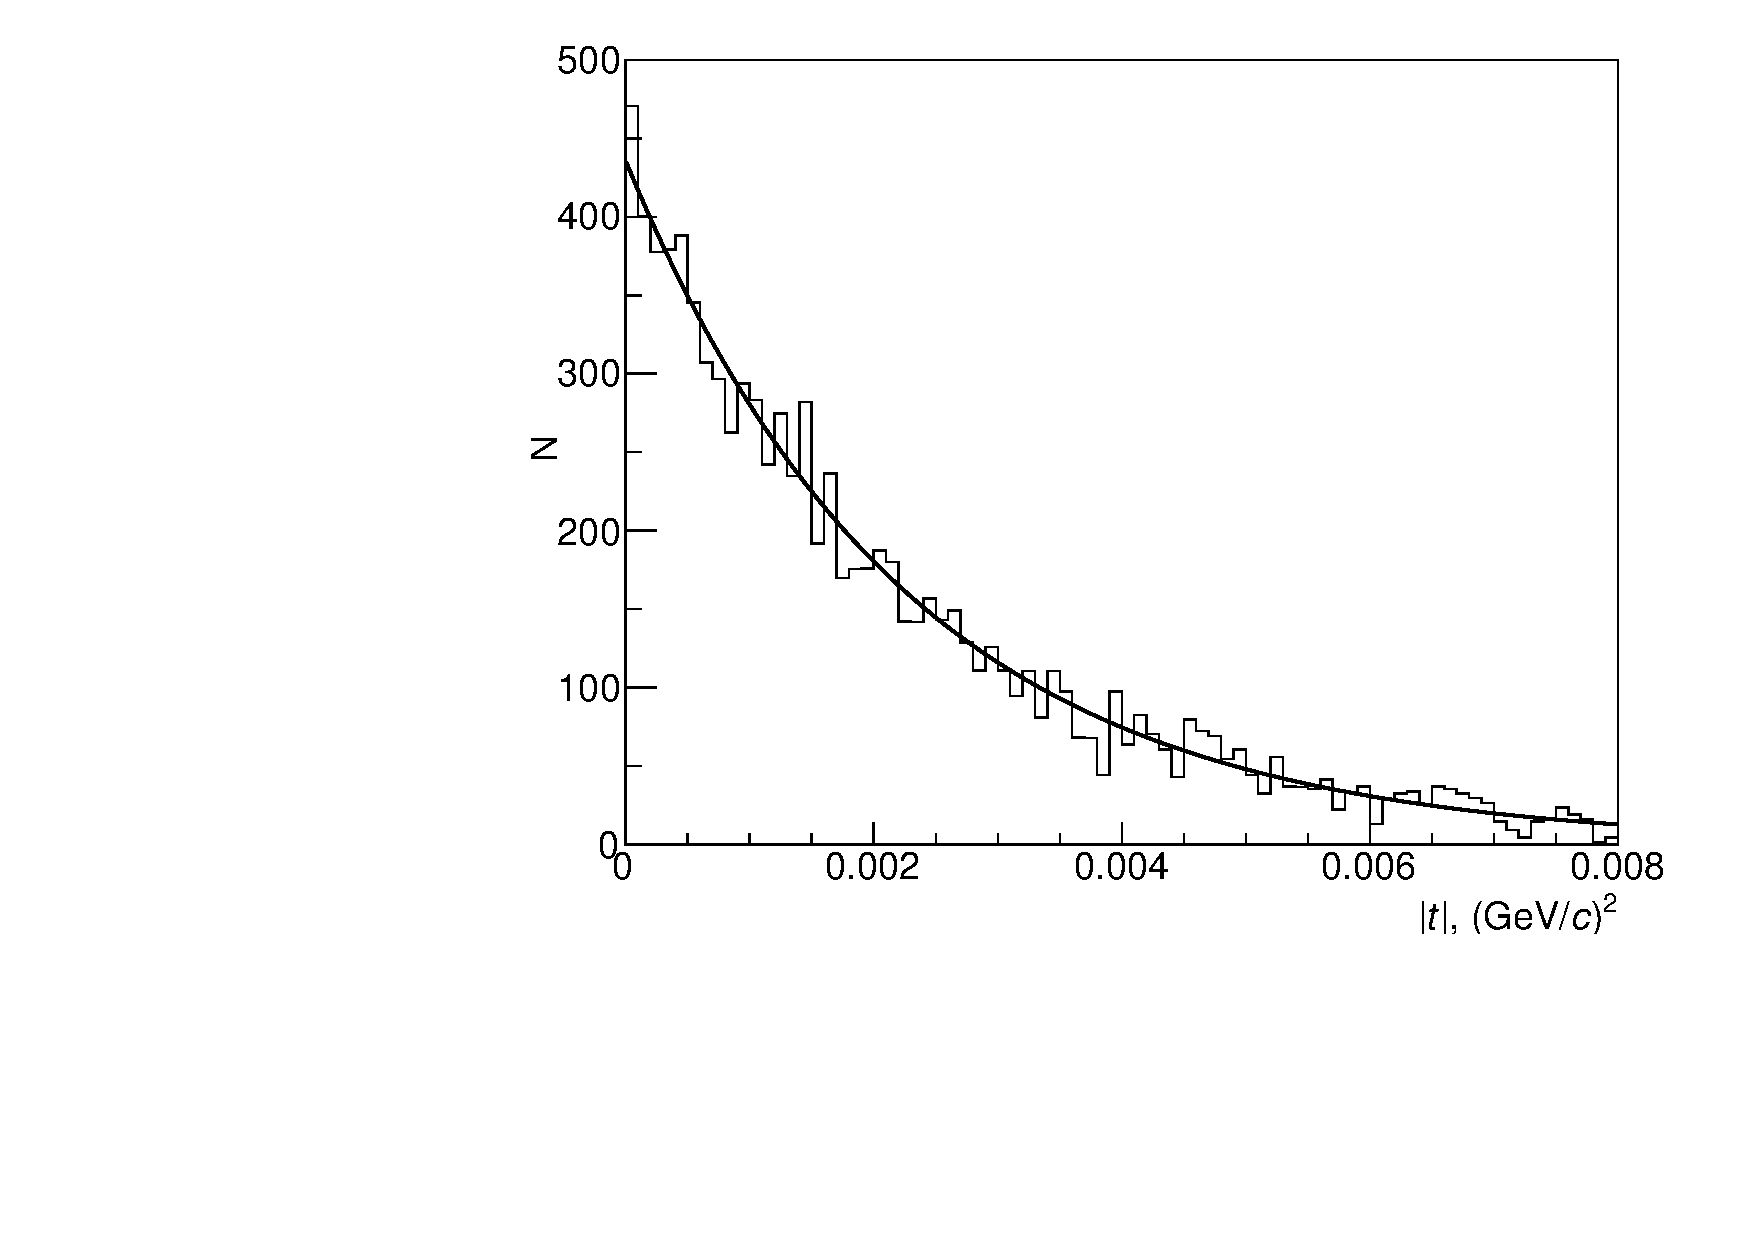
\includegraphics[width=0.48\textwidth]{dp_dN.pdf}
%DIFDELCMD <   %%%
%DIFDELCMD < \caption{%
{%DIFAUXCMD
\DIFdelFL{Differential distribution $dN/dt$ of the }%DIFDELCMD < \dpchex %%%
\DIFdelFL{reaction. The solid
    line is approximation by Eq. }%DIFDELCMD < \eqref{eq:dndtfit}%%%
\DIFdelFL{, see details in the text.}}
  %DIFAUXCMD
%DIFDELCMD < \label{fig:dndt}
%DIFDELCMD < \end{figure}
%DIFDELCMD < 

%DIFDELCMD < %%%
\DIFdel{The cross section was calculated using the relation
}\begin{displaymath}
  \DIFdel{\sigma =
  \frac{1}{n\,lb_w}\ln\bigg(1\Big/\Big(1-\frac{N_{int}}{N_0}\Big)\bigg)\,,
}\end{displaymath}%DIFAUXCMD
\DIFdel{where $n$ is the concentration of H nuclei in cm$^{-3}$ in target, $l$ is the
target length, $b_w$ is the histogram bin width, $N_{int}$ is the number of
interactions and $N_0$ is the number of beam triggers. The number of triggers is
corrected for the efficiency of chambers.
}%DIFDELCMD < 

%DIFDELCMD < %%%
\DIFdelend The obtained charge exchange differential cross section on the deuteron at $t=0$
was compared with the available data from \np reaction at the same interpolated
energy from published data. The closest energy data comes from measurements made
at the SATURN accelerator \cite{biz75,bys78}. Unlike to the other similar
experiments, Bizard et al. \cite{biz75} used quasi monochromatic neutrons from
accelerated deuteron stripping with a momentum spread of\DIFaddbegin \DIFadd{~}\DIFaddend 5~\%. New data about
\np scattering at the momenta of incident quasi monochromatic neutrons at 1.43,
2.23 and 5.20 \GeVc have been obtained in \cite{tro14}.

The values of $(d\sigma/dt)|\,_{t=0}$ of \np reaction as a function of the
incident momenta is shown in Fig. \ref{fig:npsigma}. Each individual
differential cross sections from Bizard et al. \cite{biz75} are transformed into
$d\sigma/dt$ versus $t$ in the region of momenta 1.4~--~2.0 \GeVc and
extrapolated at each momentum to $t=0$ by fitting the expression
$d\sigma/dt = a\,\exp(b\,t + c\,t^2)$. \DIFaddbegin \DIFadd{This reference dependence has already
been used in \cite{gla08}.
}\DIFaddend 

\DIFdelbegin %DIFDELCMD < \begin{figure}[ht]
%DIFDELCMD <   %%%
\DIFdelendFL \DIFaddbeginFL \begin{figure}[h]
  \DIFaddendFL \centering
  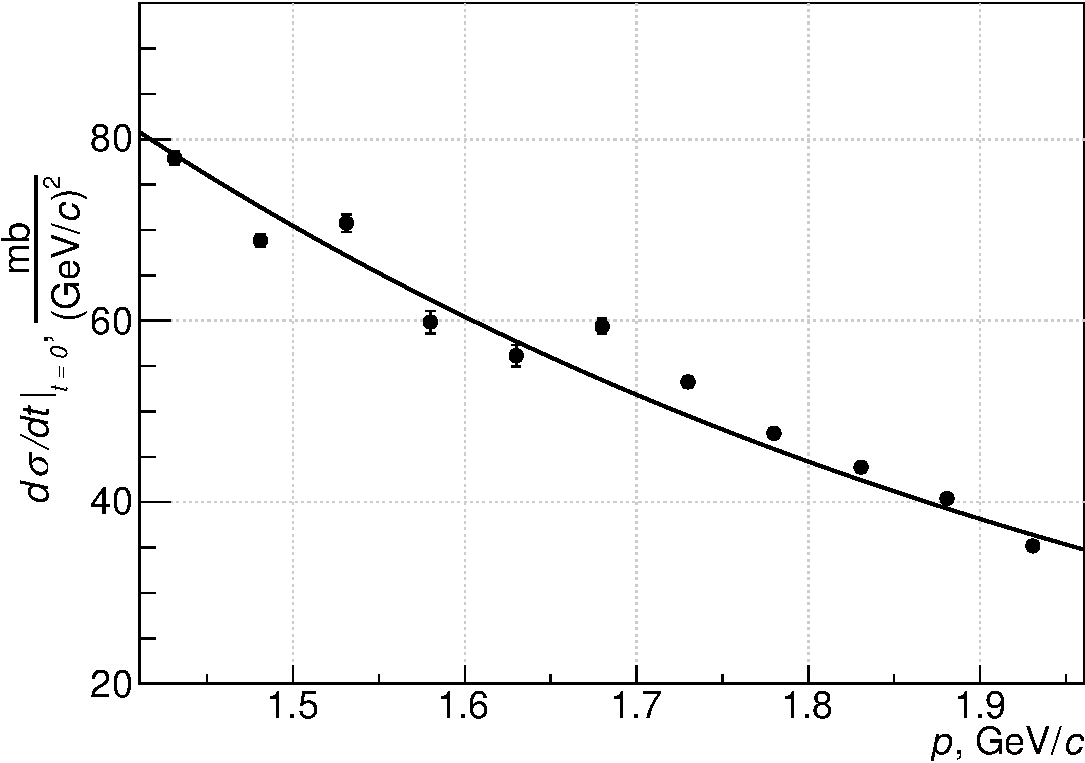
\includegraphics[width=0.48\textwidth]{np_dSigma.pdf}
  \caption{The dependence of the $(d\sigma/dt)|\,_{t=0}$ for the \np reaction on
    the beam momentum. The data points are computed from the experimental
    results \cite{biz75}. The solid curve is a simple exponential fit to the
    data points.}
  \label{fig:npsigma}
\end{figure}

To determine the $(d\sigma/dt)|\,_{t=0}$ of the \np reaction at ``our incident''
proton momentum of 1.75 \GeVc \DIFdelbegin \DIFdel{/}\DIFdelend \DIFaddbegin \DIFadd{per }\DIFaddend nucleon, an exponential fit is made to the
results of Fig. \ref{fig:npsigma}, which gives the following value of
$(d\sigma/dt)|\,_{t=0} = (48.0\,\pm\,0.2$) mb$/$(\GeVc)$^{\,2}$. The
systematical error due to fit procedure is approximately 5~\%. The obtained
value will be related to the estimated differential cross section of the quasi
elastic \dpchex charge exchange at $t=0$ from our experiment.

One can introduce the ratio of the differential cross sections for the forward
scattering (charge exchange) on the deuteron and proton
\begin{equation}
  \begin{split}
    R_{\np} &= \frac{(d\sigma/dt)_{\dpchex}}{(d\sigma/dt)_{\np}} \\
    &= 0.64 \pm 0.01\,\mathrm{(stat.)} \pm 0.04\,\mathrm{(syst.)}.
  \end{split}
\end{equation}
Under the assumption Eq. \eqref{eq:dp_23np} and Eq. \eqref{eq:np_sum} stated
above this, $R_{\np}$ can be related to
\begin{equation}
  R_{\np} = \frac{2}{3}\,\frac{(d\sigma/dt)^{SD}_{\np}}{(d\sigma/dt)_{\np}}
\end{equation}
and accordingly the \DIFdelbegin \DIFdel{value }\DIFdelend \DIFaddbegin \DIFadd{contribution }\DIFaddend of the spin-independent part\DIFdelbegin \DIFdel{of the }\DIFdelend \DIFaddbegin \DIFadd{, as a ratio of the
two parts of the }\DIFaddend elastic \np charge exchange cross section\DIFaddbegin \DIFadd{, }\DIFaddend has been obtained as
\begin{equation}
  \begin{split}
    R^{\,ID}_{\np} &= \frac{(d\sigma/dt)^{SI}_{\np}}{(d\sigma/dt)^{SD}_{\np}}
    = \frac{2}{3\,R_{\np}} \ - \ 1 \\
    &= 0.05 \pm 0.02\,\mathrm{(stat.)} \pm 0.07\,\mathrm{(syst.)}.
  \end{split}
\end{equation}
It should be emphasized that the obtained contribution, of course, depends on
the elementary \np charge exchange cross section which is taken from another
experiment and on the systematical errors of approximately 5~\% which is due to
the fit procedure. Preliminary data published in \cite{bas14,bas16} are not
contradicting the presented results.

\section{Conclusion \DIFaddbegin \DIFadd{and outlook}\DIFaddend }
The spectrometric complex \DIFdelbegin \DIFdel{has been developed on the basis of the STRELA setup }\DIFdelend \DIFaddbegin \DIFadd{STRELA has been proposed and realized }\DIFaddend to study the
charge exchange reaction in \DIFdelbegin \DIFdel{unpolarized }\DIFdelend \DIFaddbegin \DIFadd{unpola\-rized }\DIFaddend deuteron beam. The value of the charge
exchange reaction \dpchex differential cross section
$(d\sigma/dt)|\,_{t=0}=(30.56\,\pm\,0.48$) mb$/$(\GeVc)$^{\,2}$ has been
\DIFdelbegin \DIFdel{obtained }\DIFdelend \DIFaddbegin \DIFadd{established }\DIFaddend at 1.75 \DIFdelbegin \DIFdel{A }\DIFdelend \GeVc \DIFdelbegin \DIFdel{. }\DIFdelend \DIFaddbegin \DIFadd{per nucleon. This value agrees with the differential
cross section $(d\sigma/dt)|\,_{t=0}=(30.2\,\pm\,4.1$) mb$/$(}\GeVc\DIFadd{)$^{\,2}$
determined by means of the one meter hydrogen bubble chamber at 1.675 }\GeVc \DIFadd{per
nucleon. }\DIFaddend The obtained ratio of the charge exchange differential cross sections
at \DIFdelbegin %DIFDELCMD < \dpchex %%%
\DIFdel{at }\DIFdelend $t=0$ for \dpchex and \DIFaddbegin \DIFadd{that of }\DIFaddend \np \DIFdelbegin \DIFdel{reactions
}\DIFdelend \DIFaddbegin \DIFadd{reaction
}\DIFaddend $R_{\np} = 0.64 \pm 0.01\,\mathrm{(stat.)} \pm 0.04\,\mathrm{(syst.)}$ testifies
the prevailing contribution of the spin-dependent part to the \np \DIFdelbegin \DIFdel{cross section
scattering.
The obtained ratio depends on the $(d\sigma/dt)|\,_{t=0}$ the }%DIFDELCMD < \np
%DIFDELCMD < %%%
\DIFdel{reaction extracted from published data }\DIFdelend \DIFaddbegin \DIFadd{scattering}\DIFaddend .
\DIFdelbegin \DIFdel{Continuation of these researches at
}\DIFdelend \DIFaddbegin \DIFadd{This conclusion is in accordance with \cite{gla08}, where the quantities are
published with considerably large errors. For illustration of the improvement in
this experiment one can quote, \textit{e.g.}, the
$R^{\,ID}_{\np} = 0.21 \pm 0.17$ \cite{gla08} and the present ratio
$R^{\,ID}_{\np} = 0.05 \pm 0.02\,\mathrm{(stat.)} \pm 0.07\,\mathrm{(syst.)}$.
}

\DIFadd{In the region above 1 }\GeV \DIFadd{Delta-Sigma group published the
$R_{dp}(0) = (d\sigma/dt)_{\,nd} / (d\sigma/dt)_{\,np}$ ratios
\cite{sha09,sha09_2,shi11} at seven values of the neutron energies
$T_n = 0.5 - 2.0$ }\GeV\DIFadd{. Both $nd \rightarrow p(nn)$ and }\np \DIFadd{reactions were
detected in the same experiment. The reported contributions of the non-flip to
flip ratio in the }\np \DIFadd{charge exchange are estimated between 0.551 and 0.589
depending on energy. The value of $R_{dp}(0) = 0.553 \pm 0.026$ at 1.0 }\GeV
\DIFadd{\cite{sha09} is within the experimental uncertainties consistent with our
result. The experiment with monochromatic fast deuterons is more rational in
respect to the analysis of experimental data, \textit{e.g.} STRELA, because the
two secondary protons, products of the }\dpchex \DIFadd{channel, are fast moving in the
forward direction at small angles, and so they are easily detectable.
}

\DIFadd{In the works \cite{chi09,mch13} the }\dpfrag \DIFadd{reaction as was used to study
neutron proton charge exchange amplitudes on the ANKE spectrometer at the COSY
storage ring at deuteron energies of 0.6, 0.8, 0.9 and 1.135 }\GeV \DIFadd{per nucleon.
A rich set of data has been obtained on the differential cross section, vector
and tensor analyzing powers as well as on the spin correlations of the charge
exchange reaction. The whole set of data allowed to draw a conclusion on the
individual amplitudes of the }\dpchex \DIFadd{scattering. On the other hand, the
spin-independent amplitude $\alpha$, whose magnitude can only be estimated by
comparing the deuteron data with the free }\np \DIFadd{differential cross section, is
absent.
}

\DIFadd{So, to extend the studies to }\DIFaddend higher energies on STRELA setup is \DIFaddbegin \DIFadd{acceptable and
the preparation is }\DIFaddend in progress.

\begin{acknowledgements}
  The authors are grateful to the JINR VBLHEP directorate for supporting \DIFdelbegin \DIFdel{their
  }\DIFdelend \DIFaddbegin \DIFadd{the
  }\DIFaddend experiment and the Nuclotron accelerator team \DIFaddbegin \DIFadd{for providing the beam}\DIFaddend . This
  research was supported by the Ministry of Education, Science, Research and
  Sport of the Slovak Republic (VEGA Grant No.~1/0113/18).
\end{acknowledgements}

\begin{thebibliography}{99}
\bibitem{pom51}
  I. Pomeranchuk, Sov. JETF \textbf{21}, 1113 (1951)
\bibitem{chew51}
  G.F. Chew, Phys. Rev. \textbf{84}, 710 (1951)
\bibitem{mig55}
  A.B. Migdal, J. Exp. Theor. Phys. (in Russian) \textbf{28}, 3 (1955)
\bibitem{pom51_2}
  I. Pomeranchuk, Dokl. Akad. Nauk (in Russian) LXXVIII, 249 (1951)
\bibitem{lap57}
  L.I. Lapidus, J. Exp. Theor. Phys. (in Russian) \textbf{32}, 1437 (1957)
\bibitem{dea72}
  N.W. Dean, Phys. Rev. D \textbf{5}, 1661 (1972)
\bibitem{dea72_2}
  N.W. Dean, Phys. Rev. D \textbf{5}, 2832 (1972)
\bibitem{ala75}
  B.S. Aladashvili et al., Nucl. Phys. B \textbf{92}, 189 (1975)
\bibitem{ala75_2}
  B.S. Aladashvili et al., Nucl. Phys. B \textbf{86}, 461 (1975)
\bibitem{bug87}
  D.V. Bugg, C. Wilkin, Nucl. Phys. A \textbf{167}, 575 (1987)
\bibitem{led04}
  R. Lednicky, V.L. Lyuboshitz, V.V. Lyuboshitz, Proc. ISHEPP XVI, 199,
  Dubna (2004)
\bibitem{gla02}
  V.V. Glagolev et al., Eur. Phys. J. A \textbf{15}, 471 (2002)
\bibitem{gol66}
  M. Goldberger, K. Watson, Collision Theory, Wiley, New York (1966)
\bibitem{gla08}
  V.V. Glagolev et al., Cent. Eur. J. Phys. \textbf{6}, 781 (2008)
\bibitem{gla13}
  V.V. Glagolev et al., Instrum. Exp. Tech. \textbf{56}, 387 (2013)
\bibitem{sha09}
  V.I. Sharov et al.\DIFaddbegin \DIFadd{, }\DIFaddend Eur. Phys. J. A \textbf{39}, 267 (2009)
\bibitem{sha09_2}
  V.I. Sharov et al., Phys. At. Nucl. \textbf{72}, 1007 (2009)
\bibitem{shi11}
  R.A. Shindin et al., Phys. Part. Nucl. Lett. \textbf{8}, 90 (2011\DIFaddbegin \DIFadd{)
}\bibitem{chi09}
  \DIFadd{D. Chiladze et al., Eur. Phys. J. A \textbf{40}, 23 (2009)
}\bibitem{mch13}
  \DIFadd{D. Mchedlishvili et al., Eur. Phys. J. A \textbf{49} (2013}\DIFaddend )
\bibitem{biz75}
  G. Bizard et al., Nucl. Phys B \textbf{85}, 14 (1975)
\bibitem{bys78}
  J. Bystricky, F. Lehar, Nucleon-Nucleon Scattering data, Karlsruhe:
  Fachinformationszentrum, 521, (1978)
\bibitem{tro14}
  Yu.A. Troyan et al., Phys. Part. Nucl. Lett. \textbf{11}, 101 (2014)
\bibitem{bas14}
  S.N. Basilev et al., PoS (Baldin ISHEPP XXII), 137, 2014
\bibitem{bas16}
  S.N. Basilev et al., J. Phys. Conf. Ser. \textbf{678}, 012040, 2016
\end{thebibliography}

\end{document}
